%
% komplexitaet.tex -- Kapitel ueber Komplexitaetstheorie
%
% (c) 2011 Prof Dr Andreas Mueller, Hochschule Rapperswil
%
\chapter{Komplexitätstheorie\label{chapter-komplexitaet}}
\lhead{Komplexitätstheorie}
\rhead{}
Im Kapitel \ref{chapter-entscheidbarkeit} wurde untersucht, ob ein
Problem überhaupt mit einer Turingmaschine lösbar ist. Die
Effizienz der gewonnenen Algorithmen spielte keine Rolle.
In diesem Kapitel soll die Laufzeit eines Algorithmus genauer
untersucht werden. Dabei sind nur Unterscheidungen interessant,
die unabhängig von den speziellen Fähigkeiten der verwendeten
Maschine sind, nur so lassen sich allgemeingültige Aussagen
ableiten, die für jede Art von Computer gelten. Die absolute Laufzeit
ist daher kein brauchbares Kriterium, sie hängt zu stark
von individuell verschiedenen Parametern wie Taktrate, Wortbreite,
Instruktionssatz etc.~ab. 

Sobald ein geeignetes Kriterium gefunden werden kann, kann man
die Sprachen in ``leicht'' und ``schwierig'' zu entscheidende 
unterteilen. Dabei kristallisiert sich eine Klasse von
Problemen heraus, die von nichtdeterministischen Turingmaschinen
gerade noch gelöst werden können, die aber für grosse
Probleme ausserhalb der Reichweite von deterministischen Turingmaschinen
sind. Es scheint, dass diese Kluft nicht überbrückt werden kann.

Für die Praxis bedeutet dies, dass einige Probleme mit effizienten
Algorithmen gelöst werden können, während für andere 
keine effizienten Algorithmen möglich sind. Der Praktiker wird daher
das Problem einschränken müssen, denn oft lassen sich solche
Probleme unter zusätzlichen Bedingungen effizient lösen.
Voraussetzung ist natürlich, dass er Probleme diesen beiden
Klassen zuordnen kann.

%
% koufzeitmplexitaet.tex -- Laufzeitkomplexität
%
% (c) 2011 Prof Dr Andreas Mueller, Hochschule Rapperswil
%
\section{Laufzeitkomplexität}
\rhead{Laufzeitkomplexität}
\index{Laufzeitkomplexität}%
\subsection{Inputlänge}
\index{Inputlänge}%
Wenn die absolute Laufzeit eines Algorithmus nicht als Mass für
die Komplexität eines Problems dienen kann, dann vielleicht
wenigstens die Abhängigkeit der Laufzeit von der Grösse des
Problems.
Da wir unter Problemen immer ihre Übersetzung in ein
Sprachproblem verstehen, haben wir für die Grösse des Problems
ein Mass: die Länge des Wortes, welches das Problem beschreibt.

Als Beispiel betrachten wir das Problem
\index{PRIME@\textsl{PRIME}}%
\[
\text{\textsl{PRIME}}=\{ n\;|\; \text{$n\in\mathbb N$ und $n$ ist prim}\}.
\]
Es ist entscheidbar, man kann zum Beispiel alle Teiler durchtesten,
das ist mit $n$ Tests möglich.
Ein Entscheider ist also eine Turingmaschine,
der man die Zahl $n$ auf das Band schreibt, und die Turingmaschine
stellt dann fest, ob die Zahl eine Primzahl ist.
Die Zahl $n$ muss als String auf das Band geschrieben werden.
Dazu ist eine Codierung
zu wählen, üblicherweise wird dies eine Zifferndarstellung in
irgendeiner Basis $b$ sein.
Zur Darstellung der Zahl $n$ in Basis $b$
sind $l=\lfloor \log_bn\rfloor+1$ Zeichen notwendig.

Man könnte aber auch die unäre Darstellung verwenden, also so viele
$0$ auf das Band schreiben, wie die Zahl $n$ angibt.
In dieser Codierung
ist also der Input wesentlich länger, nämlich $l=n$.
Für die Beurteilung der
Komplexität kann also die Codierung des Inputs durchaus einen
merklichen Einfluss haben.
Nehmen wir an, der Algorithmus hat
eine Laufzeit proportional zu $n$, dann wächst die Laufzeit im
zweiten Fall proportional zur Inputlänge $l$, im ersten Fall
aber wächst die Laufzeit mit $b^l$.
Man kann also Algorithmen
nur vergleichen, wenn man die gleiche Inputcodierung verwendet.

\subsection{Laufzeit}
\index{Laufzeit}%
Sei jetzt also eine Turingmaschine $M$ gegeben, die ein Entscheider
ist.
Für jedes Inputwort $w$ wird die Maschine eine gewisse Zeit
laufen und dann im Zustand $q_{\text{accept}}$ oder $q_{\text{reject}}$
anhalten.
Die Anzahl der Rechenschritte, die die Maschine auf dem
Inputwort $w$ benötigt, bezeichnen wir mit $t(w)$.
Die maximale Laufzeit, die für Inputwörter der Länge nicht
grösser als $n$ benötigt wird, bezeichnen wir mit $t(n)$,
\[
t(n)=\max \{ t(w)\;|\; |w|\le n\}.
\]
Der absolute Wert von $t(n)$ ist nicht interessant, da er sich
selbst unter trivialen Veränderungen der Turingmaschine verändern
kann.
Das Verhalten von $t(n)$ für grosse $n$ hingegen scheint
wesentlich robuster zu sein, es interessiert also nur noch, wie
sich verschiedene Funktionen zueinander verhalten, wenn man $n\to\infty$
streben lässt.
Falls wir die Turingmaschine angeben wollen, deren
Laufzeit bestimmt wird, schreiben wir sie als Index zu $t$: $t_M(n)$.

\begin{definition}
Sind $f$ und $g$ Funktionen $\mathbb N\to\mathbb R^+$, dann ist
$f(n)=O(g(n))$, falls es eine Konstante $c$ und ein $n_0\in\mathbb N$
gibt mit
\[
f(n)\le cg(n)\quad \forall n\in\mathbb N\text{ mit } n > n_0.
\]
Es ist $f(n)=O(g(n))$ wenn 
\begin{equation}
\lim_{n\to\infty}\frac{f(n)}{g(n)}=0.
\label{oquotientlimit}
\end{equation}
\end{definition}
\index{Laufzeit!polynomielle}%
Man beachte, dass für $f(n)=O(g(n))$ die Ungleichung $f(n)\le
cg(n)$ nicht für alle $n$ gelten muss, insbesondere spielen kleine
Werte von $n$ keine Rolle, es interessiert uns nur das Verhalten
bei grossen Werten von $n$.
Und auch für $f(n)=O(g(n))$ sind die kleinen Werte von $n$ nicht
von Bedeutung, die Funktionswerte für kleine $n$ haben keinen
Einfluss auf den Grenzwert des Quotienten (\ref{oquotientlimit}).

Die Funktion $g$ muss offenbar nicht sonderlich genau bekannt
sein.
Ist $g$ zum Beispiel ein Polynom, interessiert nur noch
die höchste Potenz.
Es gilt ja zum Beispiel
$ n^r\le n^k $ für jeden Exponenten $r<k$, und damit
$n^r=O(n^k)$.
Ausserdem ist $an^r=O(n^k)$, und damit
für $f(n)=a_0+a_1n+a_2n^2+\dots+a_{k-1}n^{k-1}+a_nn^k$ auch
$ f(n)=O(n^k) $.
Somit genügt es bei Polynomen für $g$ die
höchste Potenz anzugeben.

\begin{beispiel}
Für das früher genannte Beispiel \textsl{PRIME} wurde 2004 etwas
überraschend ein Algorithmus mit
polynomieller Laufzeit gefunden \cite{skript:aks}.
\end{beispiel}

\subsection{Varianten von Turingmaschinen}
Wieviel schneller arbeitet eine Turingmaschine mit mehreren Bändern 
gegenüber einer Standardturingmaschine? Wieviel schneller ist eine
nichtdeterministische Turingmaschine gegenüber einer deterministischen?

\begin{satz}
\index{Turing-Maschine!mit mehreren Bändern}%
Eine Turingmaschine mit mehreren Bändern und Laufzeit $t(n)$ kann
in Laufzeit $O(t(n)^2)$ auf einer Standardturingmaschine
simuliert werden.
\end{satz}

\begin{proof}[Beweis]
In Satz \ref{mehrbandturingmaschine} wurde beschrieben, wie man eine
Turingmaschine mit mehreren Bändern auf einer Turingmaschine mit
einem einzigen Band simulieren kann.
Dabei ist für jeden der
$t(n)$ Berechnungsschritt ein Durchgang durch das Band nötig, bei
dem die Turingmaschine die Inhalte der markierten Felder zusammensammelt,
um dann die notwendigen Änderungen zu bestimmen.
Die Änderungen
auf dem Band einzutragen erfordert dann nochmals einen Durchgang
durch das Band.

Wir nehmen an, dass $t(n)\ge n$, denn sonst könnte die
Turingmaschine nicht einmal ihren Input vollständig lesen.
Der tatsächlich benutzte Teil des Bandes kann dann nicht länger sein
als $t(n)$.
Zusammen mit den $t(n)$ Durchläufen erhalten wir
die Erkenntnis,
dass die simulierte Turingmaschine die Laufzeit $O(t(n)^2)$ hat.
\end{proof}

Einen wesentlichen Unterschied der Laufzeit erwarten wir aber
bei nichtdeterministischen Turingmaschinen.
Die Berechnung in einer nichtdeterministischen Turingmaschine
kann ja auf ganz verschiedenen Wegen stattfinden, wovon
einer gefunden werden muss, der akzeptiert.
Wenn eine simulierende
Turingmaschine alle Wege durchprobiert, spielt die Laufzeit auf
demjenigen Weg, der am längsten braucht, eine wesentliche Rolle.

\begin{definition}
\index{Laufzeit!einer nichtdeterministischen Turingmaschine}%
Sei $N$ eine nicht deterministische Turingmaschine, die auch ein
Entscheider ist.
Dann ist ihre Laufzeit $t(n)$ die maximale Anzahl
von Schritten, die jede mögliche Berechnung auf einem Input der
Länge $\le n$ braucht.
\end{definition}

\begin{satz}
\label{exponentialtime}
Eine nichtdeterministische Turingmaschine mit Laufzeit $t(n)$
kann in Laufzeit $2^{O(t(n))}$
auf einer deterministischen Turingmaschine simuliert werden.
\end{satz}

\begin{proof}[Beweis]
In Satz \ref{nichtdeterministischeturingmaschine} wurde gezeigt,
wie man eine nichtdeterministische Turingmaschine auf einer
Mehrband-Maschine simulieren kann.
Da wir im vorliegenden Fall
sogar einen Entscheider haben, können wir den Algorithmus noch
etwas vereinfachen.
Wir verwenden Band~1 wieder für den Input,
Band~2 als Arbeitsband für die simulierte Turingmaschine und
Band~3 als Steuerband für die nichtdeterministischen
Entscheidungen.

Wir müssen ausrechnen, wie sich die Simulation auf die 
Gesamtlaufzeit auswirkt.
Jeder Berechnungspfad der simulierten
nichtdeterministischen Turingmaschine hat eine Laufzeit nicht
länger als $t(n)$.
Die Erzeugung der nächsten möglichen
Berechnungsgeschichte auf Band~3 kann in einem Durchgang
durch Band~3 erfolgen, braucht also Zeit $O(t(n))$.
Die Anzahl der Berechnungsgeschichten ist $|Q\times \Gamma|^{t(n)}$,
also von der Form $c^{t(n)}$.
Im schlimmsten Fall ist die
Laufzeit dieses Algorithmus also
\[
c^{t(n)}(t(n) + O(t(n)))
=
2^{t(n) \log_2 c+ \log_2(O(t(n)))}
=
2^{O(t(n))}.
\]
\end{proof}
\subsection{Wie langsam ist exponentielle Laufzeit?}
\index{Laufzeit!exponentielle}%
Satz \ref{exponentialtime} zeigt, dass zur Simulation eines
nichtdeterministischen Automaten eine exponentiell längere
Zeit nötig ist, als die nichtdeterministische Maschine
benötigt hätte.
Aber wieviel langsamer ist das?
Zunächst ist für jeden Exponenten $k$
\[
\lim_{n\to\infty}\frac{2^{n}}{n^k}=\infty,
\]
$2^n$ wächst also schneller als jedes Polynom.
Setzen wir $t=n^r$, dann ist auch
\[
\lim_{n\to\infty}\frac{2^{n^r}}{n^k}
=
\lim_{t\to\infty}\frac{2^t}{t^{k/r}}
=
\infty,
\]
wie zu erwarten war, wächst $2^{n^k}$ noch schneller.
Da nur schon für das Lesen des Input $n$ Schritte notwendig sind,
spielt es gar keine Rolle, wie effizient der Algorithmus der
nichtdeterministischen Turingmaschine ist, es ist unmöglich,
je polynomielle Laufzeit zu erreichen.

Aber wie gross ist denn nun exponentielle Laufzeit?
Nehmen wir an,
wir hätten einen Algorithmus mit Laufzeit $n^k$.
Vergrössert
man die Input-Länge um $1$ Zeichen, ändert sich die Laufzeit um
\[
\frac{(n+1)^k}{n^k}
=
1+\frac{k}{n} +\dots,
\]
die relative Zunahme wird also immer kleiner.
Bei einer Verdoppelung
der Inputlänge wird die Laufzeit mit dem Faktor $2^k$ multipliziert.
Ganz anders bei exponentieller Laufzeit.
Erhöht man die Inputlänge um $1$, wird die Laufzeit mit einem
konstanten Faktor multipliziert.
Und die Verdoppelung von $n$
quadriert die Laufzeit.
Ausgehend von einer angenommenen
Zeit pro Schritt von einer Nanosekunde, ergeben sich
für die Laufzeit eines Algorithmus
mit polynomieller Laufzeit, genauer mit $n^5$ und exponentieller Laufzeit,
genauer mit $2^n$ die Werte in Tabelle~\ref{laufzeittabelle}.
\begin{table}
\begin{center}
\begin{tabular}{|l|rr|}
\hline
$n$&$n^5$&$2^n$\\
\hline
  1&             1ns&             2ns\\
  2&            32ns&             4ns\\
  4&       1.0$\mu$s&            16ns\\
  8&      32.7$\mu$s&           256ns\\
 16&           1.0ms&      65.5$\mu$s\\
 32&          33.5ms&           4.3ms\\
 64&            1.0s&       584 Jahre\\
128&           34.4s& $10^{21}$ Jahre\\
\hline
\end{tabular}
\end{center}
\caption{Polynomielle und exponentielle Laufzeit\label{laufzeittabelle}}
\end{table}
Die Zeit von $10^{21}$ Jahren entspricht dem 78 Milliardenfachen des
Alters des Universums.
Grosse Probleme mit exponentieller Laufzeit
sind also schlicht unlösbar, während selbst relativ grosse
polynomielle Laufzeiten durchaus im Bereich des erreichbaren sind.
Der Unterschied zwischen polynomieller und exponentieller Laufzeit
ist also für grosse Inputlänge der Unterschied zwischen lösbaren und
unlösbaren Problemen.


%
% pnp.tex -- Klassen P und NP
%
% (c) 2011 Prof Dr Andreas Mueller, Hochschule Rapperswil
%
\section{Klassen P und NP}
\index{Klasse P}%
\rhead{Klassen P und NP}
\subsection{Klasse P}
Bei der Simulation einer Turingmaschine mit mehreren Bändern
auf einer Standardmaschine wird die Laufzeit im schlimmsten
Fall quadriert. Die Funktion $t_M(n)$ ist also keine Invariante
in der Menge der entscheidbaren Sprachen. Für das gleiche Problem kann
je nach eingesetztem Maschinentyp ein völlig anderes Laufzeitverhalten
beobachtet werden. 

Erhalten bleibt aber die Eigenschaft der Funktion $t_M(n)$, 
polynomiell zu sein. Simuliert man eine Turingmaschine $M_1$ mit
mehreren Bändern auf einer Standardturingmaschine $M_2$,
dann ist $t_{M_2}=O(t_{M_1}(n)^2)$.
Wenn also $t_{M_1}(n)=O(n^k)$ ist, dann ist $t_{M_2}(n)=O(n^{2k}).$
Beide Maschinen haben eine Laufzeit, die durch ein Polynom beschränkt
sind.

\begin{definition}
\index{Klasse P}%
Die Klasse $P$ besteht aus den Sprachen, die mit einem Entscheider
mit polynomieller Laufzeit entschieden werden können.
\end{definition}

\subsection{Beispiele von Sprachen in P}
\index{Sprachen!kontextfreie}%
\begin{satz}
Kontextfreie Sprachen sind in P.
\end{satz}

Der Satz besagt, dass es zu jeder kontextfreien Sprache eine
Turingmaschine gibt, die die Zugehörigkeit eines Wortes zur
Sprache in einer Zeit entscheiden kann, die polynomiell ist in
der Länge des Wortes.

\begin{proof}[Beweis]
Der CYK-Algorithmus aus Satz \ref{cyk-algorithm}
kann in Zeit $O(n^3)$ durchgeführt werden.
\end{proof}

Sei $G$ ein gerichteter Graph und $s$ und $t$ zwei Vertizes
des Graphen. Das Pfad-Problem fragt, ob es einen von $s$ nach $t$
führend Pfad in dem Graphen gibt. Übersetzt in ein Spracheproblem
liefert es uns den folgenden Satz.

\begin{satz}
\index{PATH@\textsl{PATH}}%
Die Sprache
\[
\text{\textsl{PATH}}
=\{
\langle G,s,t\rangle
\;|\;\text{$G$ ist ein gerichteter Graph mit einem Pfad von $s$ nach $t$}
\}
\]
ist in P.
\end{satz}

\begin{proof}[Beweis]
\index{Markierungsalgorithmus}%
Ein Markierungsalgorithmus, der beginnend bei $s$ alle erreichbaren
Vertizes markiert, solange sich noch neue Vertizes markieren lassen,
hat polynomielle Laufzeit.
\end{proof}

\begin{satz}
\index{RELPRIM@\textsl{RELPRIME}}%
Die Sprache
\[
\text{\textsl{RELPRIME}}
=\{
\langle a,b\rangle \;|\;
\text{$a, b\in \mathbb N$ und $a$ und $b$ sind teilerfremd}
\}
\]
ist in P.
\end{satz}

\begin{proof}[Beweis]
\index{Algorithmus!euklidischer}%
Teilerfremdheit kann mit dem euklidischen Algorithmus entscheiden werden.
Dieser funktioniert wie folgt:
\begin{compactenum}
\item Wiederhole Schritte 2 und 3 bis $y=0$:
\item Weise $x$ den Wert $x\mod y$ zu
\item Vertausche $x$ und $y$
\item Gebe Resultat $x$ zurück.
\end{compactenum}
Bei diesem Algorithmus wird $x$ in jedem Schritt mindestens halbiert,
die Laufzeit ist also proportional zur grösseren der
beiden Zahlen $\log_2 a$ und $\log_2 b$, also ist die Laufzeit
polynomiell in der Inputlänge $\log_2 a+\log_2 b$.
\end{proof}

\subsection{Verifizierer}
Sprachen, die von einer nichtdeterministischen Turingmaschine
in polynomieller Zeit entschieden werden, brauchen bei der
Simulation auf einer deterministischen Turingmaschine im
schlimmsten Fall exponentiell länger. Es ist also im
Allgemeinen fast unmöglich, ein solches Problem zu lösen.

Gibt man allerdings die Lösung vor, zum Beispiel indem man
die richtigen nichtdeterministischen Entscheidungen vorgibt,
kann man die Problemlösung in polynomieller Zeit nachvollziehen.
Genau diese Idee formalisiert das Konzept des Verifizierers.

\begin{definition}
\index{Verifizierer}%
Ein Verifizierer für die Sprache $A$ ist eine Turingmaschine
$V$ mit
\[
A=\{
w\;|\;\text{$\exists c\in C^*$ so dass $V$ $\langle w,c\rangle$ akzeptiert}
\},
\]
wobei $C$ eine endliche Menge ist.
Ein Verifizierer heisst polynomiell, wenn seine Laufzeit polynomiell
ist in der Länge des Wortes $w$.
\end{definition}

Man beachte, dass die Länge von $c$ auf die Laufzeit keinen
Einfluss haben darf. Der Verifizierer muss nämlich gar nicht
den ganzen String $c$ anschauen, er muss davon nur soviel
nehmen, wie er für die Verifikation braucht. Aber natürlich
muss er den ganzen String $w$ lesen, von dessen Länge muss
die Laufzeit abhängen.

Ein Verifizierer ist erst nützlich, wenn man auch $c\in C^*$
hat. Im Falle des Akzeptanzproblems durch eine nichtdeterministische
Turingmaschine (siehe Einführungsbeispiel) kann die Folge der
nichtdeterministischen Entscheidungen in der Berechnung diese
Funktion übernehmen. Daraus schliessen wir

\begin{satz} Eine Sprache wird genau dann von einer
nichtdeterministischen Turingmaschine in polynomieller Zeit entschieden,
wenn sie einen polynomiellen Verifizierer hat.
\end{satz}

\begin{proof}[Beweis]
Bereits gezeigt haben wir, dass eine nichtdeterministisch in
polynomieller Zeit entscheidbare Sprache einen polynomiellen Verifizierer hat.
Es ist also
nur noch zu klären, dass auch das Umgekehrte gilt, dass also eine
Sprache mit einem polynomiellen Verifizierer nichtdeterministisch
in polynomieller Zeit entschieden werden kann.

Dazu verwenden wir den folgenden Entscheidungsalgorithmus:
\begin{compactenum}
\item Erzeuge nicht deterministisch $c\in C^*$.
\item Teste, ob $V$ $\langle w,c\rangle$ akzeptiert.
\item falls $V$ akzeptiert: $q_{\text{accept}}$, falls nicht:
$q_{\text{reject}}$
\end{compactenum}
Die Laufzeit dieses Algorithmus wird bestimmt von der Laufzeit von $V$,
ist also polynomiell in der Länge von $w$.
\end{proof}

\begin{beispiel}[Faktorisierung]
Die Faktorisierung eines Produktes von zwei grossen Primzahlen
gilt allgemein als schwierig. Die Sicherheit des RSA-Algorithmus,
der in zahlreichen im Internet verbreiteten kryptographischen
Protokollen verwendet wird, basiert wesentlich auf der Tatsache, dass
es sehr einfach ist, ein Produkt von zwei grossen Primzahlen zu
bilden, aber sehr viel schwieriger, aus dem Produkt die beiden
Faktoren wieder zu ermitteln.

Es geht also um die Sprache
\[
L
=
\{
n\;|\,\text{$n=pq$, wobei $p$ und $q$ Primzahlen sind}.
\}
\]
Erfahrungsgemäss ist es praktisch unmöglich, die Faktoren
einer Zahl in $n$ zu bestimmen, und damit zu entscheiden, ob
$n\in L$ ist. Kennt man jedoch einen der beiden Faktoren,
zum Beispiel $p$, dann kann man mit dem Divisionsalgorithmus
nachprüfen, ob die Division ``aufgeht'', was in einer Anzahl
von Schritten möglich ist, die proportional zur Länge von 
$n$, also zu $\log_b n$ ist. Der Test auf Rest 0 bei Teilung
durch $p$ ist also ein polynomieller Verifizierer mit $c=p$.
\end{beispiel}

\subsection{Klasse NP}
Keine Variante der Turingmaschine macht aus einem Problem,
welches sich in einer Laufzeit $2^{O(n^k)}$ entscheiden
lässt, ein Problem in $P$. Es ist daher zu vermuten,
dass die Sprachen, die nichtdeterministisch in polynomieller
Zeit entschieden werden können, eine wesentlich grössere
Klasse bilden als $P$.

\begin{definition}
\index{Klasse NP}%
Die Klasse der von einer nichtdeterministischen Turingmaschine
in polynomieller Zeit entscheidbaren Sprachen heisst NP.
\end{definition}

\begin{figure}
\begin{center}
\includegraphics{images/lang-5}
\end{center}
\caption{Jede Sprache in P ist auch in NP\label{psubsetnp}}
\end{figure}%

Insbesondere enthält NP alle Sprachen mit einem polynomiellen
Verifizierer. Es ist auch klar, dass $\text{P}\subset\text{NP}$,
siehe Abbildung \ref{psubsetnp}.
Ein offenes Problem ist jedoch, ob $\text{P}\ne \text{NP}$.
Die Bedeutung dieser Frage wird später klar werden.

\subsection{Satisfiability: \textsl{SAT}}
\index{SAT}%
\index{Satisfiability}%
Die Sprache 
\[
\text{\textsl{SAT}}=\{\varphi\;|\;\text{$\varphi$ ist eine erfüllbare logische Formel}\}
\]
ist entscheidbar. Für eine logische Formel $\varphi(x_1,\dots,x_n)$
testet man einfach alle möglichen Belegungen der Variablen $x_1,\dots,x_n$
mit Wahrheitswerten.
Dafür sind $2^n$ Verifikationen notwendig, dies ist also
bestimmt kein Algorithmus in P.

\textsl{SAT} ist aber in NP,
denn wir können einen polynomiellen Verifizierer angeben.
Der Verifizierer verlangt als Lösungszertifikate $c$ eine
Belegung der Variablen mit Wahrheitswerten $c=(x_1,\dots,x_n)$,
und überprüft, ob durch einsetzen der Werte $x_1,\dots,x_n$
die Formel $\varphi(x_1,\dots,x_n)$ wahr wird.

Eine Variante von \textsl{SAT} ist \textsl{3SAT}.
Im Gegensatz zu \textsl{SAT} enthält \textsl{3SAT}
nur Formeln in konjunktiver Normalform, und jede Klausel
enthält genau drei Terme (3cnf-Formel).
Eine typische Formel in \textsl{3SAT} ist 
\[
\varphi=(x_1\vee x_2\vee x_3)\wedge (\bar x_1\vee x_3\vee \bar x_4)\wedge
	(x_1\vee x_3\vee x_5).
\]
Die Sprache \textsl{3SAT} ist
\[
\text{\textsl{3SAT}} =\{\varphi\;|\; \text{$\varphi$ ist eine erfüllbare 3cnf-Formel}\}.
\]
Wie \textsl{SAT} ist \textsl{3SAT} in NP.

\subsection{Existenz von Cliquen: \texorpdfstring{$k$}{k}-\textsl{CLIQUE}}
\begin{figure}
\begin{center}
%\includegraphics[width=0.6\hsize]{images/comp-1}
\includegraphics[width=0.35\hsize]{images/comp-1}
\end{center}
\caption{Graph mit sechs Knoten, keiner 4-Clique, aber
vier 3-Cliquen\label{6graph}}
\end{figure}%
\begin{figure}
\begin{center}
\begin{tabular}{cccc}
\includegraphics[width=0.35\hsize]{images/comp-2}&%
\includegraphics[width=0.35\hsize]{images/comp-3}\\
\includegraphics[width=0.35\hsize]{images/comp-4}&%
\includegraphics[width=0.35\hsize]{images/comp-5}
\end{tabular}
\end{center}
\caption{3-Cliquen des Graphen von Abbildung~\ref{6graph}}
\end{figure}%
\index{Clique}%
\index{Clique@$k$-Clique}%
\index{Cliquen-Problem}%
\index{CLIQUE@\textsl{CLIQUE}}%
Eine $k$-Clique in einem Graph $G$ ist eine Menge von $k$
Ecken des Graphen so, dass in $G$ jede Ecke der Teilmenge mit
jeder anderen Ecke verbunden ist. Im umgangssprachlichen Gebrauch
ist eine Clique eine Gruppe von Leuten, in der jeder jeden kennt.

Das Cliquen-Problem
\[
\text{$k$-\textsl{CLIQUE}} = \{ \langle G\rangle\;|\;
\text{$G$ ist ein Graph mit einer $k$-Clique}\}
\]
ist entscheidbar. Man probiert alle möglichen $k$-elementigen
Teilmengen der Ecken des Graphen durch, ob sie eine Clique
bilden. Da Zahl der Teilmengen ist $\binom{n}{k}$, wenn $n$
die Zahl der Ecken ist, und $\binom{n}{k}$ von der Grössenordnung
$O(n^k)$ ist, ist dieser Algorithmus nicht in P.

Das Cliquen-Problem ist aber in NP. Dazu muss wieder ein
Verfizierer angegeben werden. Als Lösungszertifikat verlangt
der Verifizierer die Menge $c=\{v_1,\dots,v_k\}$ der
Vertizes, die angeblich eine $k$-Clique bilden. Dann testet
er jedes Paar von Vertices in $c$ daraufhin, ob sie in $G$
verbunden sind. Dies sind weniger als $k^2$ Tests die nicht
weniger Aufwand als die Grösse des Graphen brauchen, die
Komplexität dieses Algorithmus ist also $O(n)$, das
Cliquen-Problem ist in NP.

\subsection{Färbeproblem: \texorpdfstring{$k$}{k}-\textsl{VERTEX-COLORING}}
\index{F\ärbeproblem}%
\begin{figure}
\begin{center}
\begin{tabular}{ccc}
\includegraphics{images/comp-6}&
\qquad&\qquad
\includegraphics{images/comp-7}
\end{tabular}
\end{center}
\caption{Zum Färbeproblem: der Graph links kann mit drei Farben
eingefärbt werden, der Graph rechts braucht vier verschiedene Farben
\label{vertex-coloring-examples}}
\end{figure}%
\index{VERTEX-COLORING@\textsl{VERTEX-COLORING}}%
Man sagt, die Vertizes eines Graphen $G$ können mit $k$ Farben
eingefärbt werden, wenn sich für jeden Vertex eine der $k$ Farben
wählen lässt, so dass nie zwei durch eine Kante verbundene Vertizes
die gleiche Farbe bekommen.

Das Färbe-Problem 
\[
\text{$k$-\textsl{VERTEX-COLORING}}
=
\{
\langle G\rangle\;|\;
\text{$G$ ist ein mit $k$ Farben einfärbbarer Graph}\}
\}
\]
ist entscheidbar. Man kann alle $k^n$ möglichen Färbungen
($n$ die Anzahl der Vertizes) durchtesten, ob sie die Bedingung
erfüllen, dass verbundene Vertizes nicht die gleiche Farbe haben
dürfen.

$k$-\textsl{VERTEX-COLORING} ist in NP, denn ein polynomieller Verifizierer
wird als Lösungszertifikat die Farbzuordnung $c=(c_1,\dots,c_n)$ der
Ecken $1,\dots,n$ des Graphen verlangen, und kann damit in polynomieller
Zeit prüfen, ob die Bedingung verschiedener Farbe an den Enden
jeder Kante erfüllt ist.


%
% reduktion.tex -- Reduktion
%
% (c) 2019 Prof Dr Andreas Müller, Hochschule Rapperswil
%
\section{Reduktion}
\index{Reduktion}%
\rhead{Reduktion}
Im letzten Abschnitt wurde die Entscheidbarkeit der Sprache $L$
auf das Akzeptanzproblem in dem Sinne zurückgeführt, dass
aus einem Entscheider für $L$ ein Entscheider für das Akzeptanzproblem
konstruiert wurde.
Die Nichtentscheidbarkeit des Akzeptanzproblems
hat dann gezeigt, dass auch $L$ nicht entscheidbar sein kann.

Dieses Vorgehen funktioniert in sehr vielen Fällen, wir wollen es
daher etwas abstrakter formulieren und damit die Anwendung in weiteren
Beispielen vereinfachen.
Gleichzeitig ermöglicht es uns, die
Sprachen mindestens teilweise nach ihrer Schwierigkeit, sie zu entscheiden,
anzuordnen.

\subsection{Reduktionsabbildung}
\index{Reduktionsabbildung}%
\begin{figure}
\begin{center}
%\includegraphics[width=\hsize]{images/red-1}
\includegraphics{images/red-1}
\end{center}
\caption{Reduktionsabbildung $f\colon A\to B$.\label{reduktionsabbildung}}
\end{figure}
Wir möchten zwei verschiedene Sprachen 
$A$ und $B$ 
vergleichen.
Dazu bilden wir Wörter von der einen Sprache in
die andere Sprache ab, wir brauchen also eine Abbildung, die
$f\colon\Sigma^*\to \Sigma^*$, die $A$ in $B$ überführt,
d.\,h.
\[
w\in A\Leftrightarrow f(w)\in B.
\]
Diese Abbildung hilft uns allerdings nur dann, Entscheidbarkeitsfragen
von $B$ nach $A$ zu transportieren, wenn sie mit einer Turingmaschine
berechnet werden kann.
Wir definieren daher

\begin{definition}
\index{berechenbar}%
Eine Abbildung $f\colon \Sigma^*\to \Sigma^*$ heisst berechenbar wenn es eine
Turingmaschine gibt, die auf jedem Input $w\in \Sigma^*$ anhält
und ausschliesslich das Wort $f(w)$ auf dem Band zurücklässt.
\end{definition}

\begin{definition}
\index{Reduktion}%
Eine Sprache $A$ ist reduzierbar auf die Sprache $B$, in Zeichen
\[
A\le B
\]
wenn es eine
berechenbare Abbildung $f\colon \Sigma^*\to \Sigma^*$ gibt, mit
\[
w\in A\Leftrightarrow f(w)\in B.
\]
Wir schreiben dafür auch
\[
f\colon A\le B.
\]
\end{definition}
Die Schreibweise $A\le B$ soll ausdrücken, dass die Sprache $A$ ``leichter''
zu entscheiden ist als die Sprache $B$.
Die nachfolgenden zwei Sätze
zeigen, dass diese Leseart berechtigt ist.

\begin{satz}
Seien $A\le B$ Sprachen.
Ist $B$ entscheidbar, dann auch $A$.
\end{satz}

\begin{proof}[Beweis]
Ist $B$ entscheidbar, dann gibt es einen Entscheider für $B$, also
eine Turingmaschine $M$, die auf jedem Inputwort anhält, und
entscheidet, ob es zu $B$ gehört.
Daraus können wir jetzt einen Entscheider für $A$ konstruieren.
Um zu entscheiden, ob $w\in A$
ist, verwenden wir den folgenden Algorithmus $M'$ mit Input
$w$:
\medskip
\begin{compactenum}
\item Berechne $f(w)$, dafür gibt es wegen $A\le B$ eine Turingmaschine.
\item Verwende den Entscheider $M$ um zu entscheiden, ob $f(w)\in B$.
\item Falls $M$ akzeptiert ist $f(w)\in B\Rightarrow w\in A$
\item Falls $M$ nicht akzeptiert ist $f(w)\not\in B\Rightarrow w\not\in A$.
\end{compactenum}
\medskip
$M'$ ist offenbar ein Entscheider für $A$, also ist $A$ entscheidbar.
\end{proof}

Die Kontraposition dieser Aussage ist
\begin{satz}
Ist $A\le B$ und $A$ nicht entscheidbar, dann ist auch $B$ nicht
entscheidbar.
\end{satz}
Damit haben wir eine Methode, um Sprachen als nicht entscheidbar 
zu beweisen.
Wir müssen nur eine Abbildung $f\colon \Sigma^*\to \Sigma^*$
konstruieren, wobei $A$ ein bekanntermassen nicht
entscheidbares Problem ist, und $f$ berechenbare Abbildung ist,
die die Reduktion $A\le B$ vermittelt.

\subsection{Weitere nicht entscheidbare Sprachprobleme}
\index{Halteproblem}%
\begin{satz} Das Halteproblem
\[
\text{\it HALT}_{\text{TM}}=\{\langle M,w\rangle\;|\;
\text{$M$ ist eine TM und $M$ hält auf Input $w$}\}
\]
\index{HALTTM@$\textit{HALT}_{\text{TM}}$}%
ist nicht entscheidbar.
\end{satz}

\begin{proof}[Beweis]
Wir konstruieren eine Reduktion
$
A_{\text{TM}}
\le
\text{\it HALT}_{\text{TM}}
$.
Die Reduktion muss aus einer TM $M$ und einem Inputwort $w$ eine
neue TM $S$ und ein Inputwort $w$ machen, so dass $S$ auf
Input $w$ genau dann hält, wenn $M$ das Wort $w$ akzeptiert.
Die Abbildung $f$ ist also
\[
f\colon 
A_{\text{TM}}
\le
\text{\it HALT}_{\text{TM}}
\colon
\langle M,w\rangle\mapsto \langle S,w\rangle.
\]
$S$ konstruieren wir wie folgt:
\medskip
\begin{compactenum}
\item lasse $M$ laufen auf Input $w$
\item falls $M$ das Wort $w$ erkennt: $q_{\text{accept}}$
\item falls $M$ verwirft: beginne eine Endlosschleife
\end{compactenum}
\medskip
Offenbar ist
$\langle S,w\rangle\in \text{\it HALT}_{\text{TM}}$
genau dann, wenn $\langle M,w\rangle\in A_{\text{TM}}$.
Wir haben also
\[
\langle M,w\rangle\in A_{\text{TM}}
\qquad
\Leftrightarrow
\qquad
\langle S,w\rangle=f(\langle M,w\rangle)
\in \text{\it HALT}_{\text{TM}}.
\]
Somit ist 
$A_{\text{TM}}\le\text{\it HALT}_{\text{TM}}$, und da
$A_{\text{TM}}$ nicht entscheidbar ist, ist auch
$\text{\it HALT}_{\text{TM}}$ nicht entscheidbar.
\end{proof}
Statt des Anhaltens könnte man auch viele andere spezielle
Betriebszustände einer Turingmaschine als ``Haltekriterien''
heranziehen.
Dann bedeutet der Satz, dass es keinen allgemeinen
Algorithmus geben kann, der ein Stück Code inspizieren kann und
daraus ableiten kann, ob dieser Code auf einem System Schaden
anrichtet.
Echte Schadcode-Erkennung gibt es also grundsätzlich
nicht (auch wenn das Marketing-Material gewisser Produkte sich
da zu ganz erstaunlichen Aussagen versteigt).
Das beste, was man
tun kann, ist Mustererkennung (endliche Sprachen sind alle regulär).

\begin{satz}
\index{Leerheitsproblem!für Turingmaschinen}%
Das Leerheitsproblem für Turingmaschinen
\[
E_{\text{TM}}
=
\{ \langle M\rangle\;|\; \text{$M$ ist eine TM und $L(M)=\emptyset$}\}
\]
\index{ETM@$E_{\text{TM}}$}%
ist nicht entscheidbar.
\end{satz}

\begin{proof}[Beweis]
Wir möchten eine Reduktion $A_{\text{TM}}\le E_{\text{TM}}$ konstruieren.
Dazu müssen wir aus $\langle M,w\rangle$ eine Maschine $S$ konstruieren,
die genau dann kein einziges Wort akzeptiert, wenn $M$ das Wort $w$
akzeptiert.
Es ist allerdings einfacher, die Negation zu behandeln,
also zu zeigen, dass 
\[
\bar E_{\text{TM}}=
\{ \langle M\rangle\;|\; \text{$M$ ist eine TM und $L(M)\ne\emptyset$}\}
\]
nicht entscheidbar ist.
Wir brauchen dann eine Reduktion
$A_{\text{TM}}\le \bar E_{\text{TM}}$, d.\,h.~eine Maschine $S$,
die genau dann mindestens ein Wort erkennt, wenn $M$ das Wort $w$ 
erkennt.

Die Maschine $S$ muss auf beliebigen Wörtern $u$ als Input ausgeführt
werden können.
Wir könnten folgenden Algorithmus verwenden:
\medskip
\begin{compactenum}
\item Falls $u\ne w$: $q_{\text{reject}}$.
\item Lasse $M$ auf $w$ laufen.
\item Falls $M$ erkennt: $q_{\text{accept}}$.
\end{compactenum}
\medskip
Wenn $M$ das Wort $w$ erkennt, dann erkennt $S$ die Sprache 
$L(S)=\{w\}$.
Wenn $M$ das Wort $w$ nicht erkennt, ist $L(S)=\emptyset$.
Oder
\begin{align*}
M&\operatorname{erkennt}w              &&\Rightarrow&L(S)&=\{w\}\ne \emptyset
\\
M&\operatorname{erkennt}w\text{ nicht} &&\Rightarrow&L(S)&=\emptyset
\end{align*}
oder
\[
\langle M,w\rangle \in A_{\text{TM}}
\qquad
\Leftrightarrow
\qquad
\langle S\rangle = f(\langle M,w\rangle)\in
\bar E_{\text{TM}},
\]
also $A_{\text{TM}}\le \bar E_{\text{TM}}$.
\end{proof}

\begin{satz}
Es ist nicht entscheidbar, ob eine Turingmaschine eine reguläre
Sprache erkennt.
\end{satz}

\begin{proof}[Beweis]
Als Sprache formuliert möchten wir eine Reduktion 
\[
A_{\text{TM}}\le\text{\it REGULAR}_{\text{TM}}=\{
\langle M\rangle\;|\;\text{$M$ ist eine TM und $L(M)$ ist regulär}
\}
\]
\index{REGULARTM@$\textit{REGULAR}_{\text{TM}}$}%
konstruieren.
Auch in diesem Fall ist es einfacher, eine
Reduktion
\[
A_{\text{TM}}\le\overline{\text{\it REGULAR}}_{\text{TM}}
\]
zu konstruieren.

Wir müssen also eine TM $S$ konstruieren, die genau
dann eine nicht reguläre Sprache erkennt, wenn $w$ von $M$ erkannt wird.
Der folgende Algorithmus tut dies.
Auf Input $u$ geht er wie folgt
vor:
\medskip
\begin{compactenum}
\item Falls $u$ nicht von der Form $0^n1^n$ ist: $q_{\text{reject}}$
\item Lasse $M$ auf $w$ laufen.
\item Falls $M$ $w$ erkennt: $q_{\text{accept}}$
\item Falls $M$ $w$ verwirft: $q_{\text{reject}}$
\end{compactenum}
\medskip
Wegen Schritt~1 kann $S$ höchstens die Wörter der Form
$\texttt{0}^n\texttt{1}^n$ erkennen, alle anderen werden bereits in
Schritt $1$ verworfen.
Ob die Wörter 
$\texttt{0}^n\texttt{1}^n$ erkannt werden, hängt davon ab, ob $M$ das Wort
$w$ erkennt:
\begin{align*}
   M&\text{ erkennt $w$}      &
    &\Leftrightarrow&
L(S)&=\{\texttt{0}^n\texttt{1}^n\,|\, n\ge 0\}&
    &\Leftrightarrow&
    &\text{$L(S)$ nicht regulär}\\
   M&\text{ erkennt $w$ nicht}&
    &\Leftrightarrow&
L(S)&=\{\quad\}=\emptyset&
    &\Leftrightarrow&
    &\text{$L(S)$ regulär}
\end{align*}
$S$ erkennt die nicht reguläre Sprache $\{0^n1^n\;|\;n\in\mathbb N\}$
genau dann, wenn $M$ das Wort $w$ erkennt.
Die Reduktion $\langle M,w\rangle\to \langle S\rangle$ übersetzt
``erkennen'' in ``nicht reguläre Sprache erkennen'', also also $A_{\text{TM}}$
in $\overline{\textsl{REGULAR}}_{\text{TM}}$.
\end{proof}

\index{Gleichheitsproblem!für Turingmaschinen}%
\begin{satz}
Ob zwei Turingmaschinen die gleiche Sprache
\[
\text{\it EQ}_{\text{TM}}=\{
\langle M_1,M_2\rangle\;|\;\text{$M_i$ sind Turingmaschinen und $L(M_1)=L(M_2)$}
\}
\]
\index{EQTM@$\textit{EQ}_{\text{TM}}$}%
erkennen, ist nicht entscheidbar.
\end{satz}

\begin{proof}[Beweis]
Wir konstruieren eine Reduktion
$
E_{\text{TM}}\le \text{\it EQ}_{\text{TM}}
$
.
Dazu sei $M_0$ eine Turingmaschine, die jeden Input verwirft,
also $L(M_0)=\emptyset$.
Für die Abbildung $f$ verwenden wir
\[
f
\colon
E_{\text{TM}}\le \text{\it EQ}_{\text{TM}}
\colon
\langle M\rangle\mapsto \langle M,M_0\rangle
\]
Es ist $\langle M,M_0\rangle\in \text{\it EQ}_{\text{TM}}$
genau dann, wenn
$L(M)=L(M_0)=\emptyset$, also genau dann, wenn
$\langle M\rangle\in E_{\text{TM}}$.
\end{proof}

Dieser Satz hat zum Beispiel zur Folge, dass es keine zuverlässige
maschinelle
Möglichkeit gibt, herauszufinden, ob zwei Programme das gleiche tun.
Damit ist die Entscheidung, ob ein beliebiges Programm ein beliebiges
Softwarepatent verletzt, nur durch den subjektiven Prozess in Form
eines Gerichtes möglich, kann also grundsätzlich niemals objektiv sein.


%
% npcomplete.tex -- NP-vollständige Probleme
%
% (c) 2011 Prof Dr Andreas Mueller, Hochschule Rapperswil
%
\section{NP-vollständige Probleme}
\rhead{NP-vollständige Probleme}
\begin{figure}
\begin{center}
\includegraphics{images/lang-4}
\end{center}
\caption{Beziehung zwischen P, NP und NP-vollständigen Problemen.
\label{pnpnpcomplete}}
\end{figure}%
Die polynomielle Reduktion ordnet die Sprachen nach ``Schwierigkeitsgrad''
(Abbildung~\ref{pnpnpcomplete}).
Je ``grösser'' eine Sprache $B$ ist, desto mehr Sprachen $A$ gibt es
mit $A\le_P B$.
Findet man einen polynomiellen Algorithmus für $B$,
löst man damit automatisch auch $A$ für alle diese $A$.

Möchte man $\text{P} = \text{NP}$ beweisen, dann muss man nach
möglichst ``schwierigen'' Problemen suchen, also nach solchen,
deren polynomielle Lösung die polynomielle Lösung vieler anderer
Probleme nach sich ziehen würde.

\begin{definition}
\index{NP-vollständig}%
Eine Sprache $B$ heisst NP-vollständig, wenn 
\begin{compactenum}
\item $B\in\text{NP}$
\item $A\le_P B$ für alle $A\in\text{NP}$
\end{compactenum}
\end{definition}

Wenn man die polynomielle Lösung eines NP-vollständigen Problemes
findet, sind auch alle anderen Probleme in NP in polynomieller Zeit
lösbar:

\begin{satz}
Falls $B$ NP-vollständig ist und $B\in\text{P}$, dann ist
$\text{P}=\text{NP}$.
\end{satz}

\begin{proof}[Beweis]
Ist $A\in\text{NP}$, dann ist $A\le_P B$, weil $B$ NP-vollständig ist.
Nach Satz \ref{polynomiellreduction} ist dann aber auch
$A\in\text{P}$, alle Sprachen
in NP sind also auch in P, oder $\text{P}=\text{NP}$.
\end{proof}


%
% sat.tex -- SAT
%
% (c) 2011 Prof Dr Andreas Mueller, Hochschule Rapperswil
%
\section{SAT}
\rhead{SAT}
\index{Cook, Steven}%
\index{Levin, Leonid}%
Bislang ist noch nicht klar, dass es überhaupt NP-vollständige
Probleme gibt. Dies änderte sich mit dem Satz von Cook und Levin,
der beweist, dass \textsl{SAT} NP-vollständig ist.

\begin{satz}[Cook-Levin]
\label{cooklevin}
\textsl{SAT} ist NP-vollständig.
\end{satz}

\subsection{SUDOKU und SAT\label{subsection:sudoku-und-sat}}
\index{Sudoku}
Als Vorstufe der angestrebten Erkenntnis, dass sich jedes Problem auf \textsl{SAT}
reduzieren l"asst, wollen wir zeigen, dass sich die Frage nach der
L"osbarkeit eines Sudoku-R"atsels auf \textsl{SAT} reduzieren l"asst.

Ein $n$-Sudoku ist ein $n^2\times n^2$-Feld, welches mit $n^2$ verschiedenen
Zeichen aus einer Menge $\Sigma$ so gef"ullt werden muss,
dass in jeder Zeile, jeder Spalte
und in jedem der $n\times n$-Unterquadrate jedes Zeichen genau einmal
vorkommt.
Die aus R"atselspalten von Zeitungen bekannten $3$-Sudokus verwenden
die Ziffern $1$ bis $9$ f"ur $\Sigma$.
Einige der Zeichen sind bereits vorgegeben, die leeren Felder m"ussen
so gef"ullt werden, dass die Regeln nicht verletzt werden.
Abbildung~\ref{sudoku} zeigt ein l"osbares $3$-Sudoku-R"atsel.
\begin{figure}
\begin{center}
\includegraphics[width=0.4\hsize]{images/sudoku-1.pdf}
\end{center}
\caption{$3$-Sudoku, die hellen Ziffern zeigen, dass die Vorgabe (dunkle
Ziffern) erf"ullbar ist, das $3$-Sudoko ist l"osbar.\label{sudoku}}
\end{figure}
Wir schreiben
\begin{align*}
\textsl{SUDOKU}
=
\{\langle S\rangle\;|\; \text{$S$ ist ein l"osbares $n$-Sudoku}\}.
\end{align*}

Ob ein $n$-Sudoku l"osbar ist, ist sicher entscheidbar: man kann alle
$|\Sigma|^{n^2\cdot n^2}=n^{2n^4}$ m"oglichen Belegungen des Feldes mit
Zeichen durchprobieren, was aber nat"urlich exponentielle Zeit
beansprucht.

\textsl{SUDOKU} ist auch in NP, denn man kann als L"osungszertifikat
die Zeichen im vollst"andig ausgef"ullten Feld verwenden.
Zur Verifikation muss man dann nur "uberpr"ufen, ob die
vorgegebenen Zeichen richtig in die L"osung "ubernommen wurden und
ob die Sudoku-Regeln eingehalten wurden. Dies ist in Laufzeit $O(n^4)$
m"oglich, es gibt also einen polynomiellen Verifizierer.

Der Satz~\ref{cooklevin} behauptet, \textsl{SAT} sei NP-vollst"andig,
es m"usste sich also auch \textsl{SUDOKU} polynomiell auf \textsl{SAT}
reduzieren lassen:

\begin{satz} $\textsl{SUDOKU}\le_P\textsl{SAT}$.
\label{skript:satz:sudoku-sat}
\end{satz}

\begin{proof}[Beweis]
Wir m"ussen eine Reduktion konstrukieren, die jedem Sudoku-R"atsel
eine logische Formel zuordnet, welche genau dann erf"ullbar ist, wenn
das Sudoku-R"atsel l"osbar ist. Wir gehen in zwei Schritten vor. 
Zun"achst konstrieren wir eine Formel, die genau dann erf"ullbar ist,
wenn das Sudoku l"osbar ist, die aber noch keine logische Formel ist.
Im zweiten Schritt wandeln wir die Formel dann in eine "aquivalente
logische Formel um.

1.~Schritt: Sei also $S$ ein gegebenes $n$-Sudoku. Wenn das R"atsel l"osbar
ist, dann gibt es f"ur jedes Feld ein Zeichen, f"ur welches alle Sudoku-Regeln
eingehalten werden. Wir bezeichnen das Zeichen in dem Feld in Zeile $i$
und Spalte $j$ mit $z_{ij}$. F"ur einige Felder gibt es Vorgaben, die wir mit
$v_{ij}$ bezeichnen. Jetzt m"ussen die Bedingungen f"ur eine korrekte
L"osung des Sudoku formuliert werden:
\begin{compactenum}
\item {\em Vorgaben sind korrekt:} Die Vorgabe im Feld $(i,j)$ ist erf"ullt,
wenn gilt $z_{ij}=v_{ij}$. Alle Vorgaben sind erf"ullt, wenn der Ausdruck
\[
\varphi_{\text{Vorgaben}}=\bigwedge_{\text{Feld $(i,j)$ ist Vorgabefeld}}(z_{ij}=v_{ij})
\]
wahr ist.
\item {\em Zeilenbedingung:} Der Wert $z_{ij}$ in Zeile $i$ ist erlaubt,
wenn jedes andere $z_{ij}$ in der Zeile $i$ verschieden davon ist:
\[
\varphi_{\text{Zeilenbedingung $(i,j)$}}
=
\bigwedge_{k\ne j}(z_{ij}\ne z_{ik}).
\]
\item {\em Spaltenbedingung:} Der Wert $z_{ij}$ in Spalte $j$ ist erlaubt,
wenn jedes andere $z_{kj}$ in der Spalte $j$ verschieden ist:
\[
\varphi_{\text{Spaltenbedingung $(i,j)$}}
=
\bigwedge_{k\ne i}(z_{ij}\ne z_{kj}).
\]
\item {\em Unterfeld-Bedingung:} Der Wert $z_{ij}$ im $n\times n$-Unterfeld,
welches $(i,j)$ enth"alt, ist zul"assig, wenn jedes andere Zeichen im gleichen
Unterfeld davon verschieden ist:
\[
\varphi_
{\text{Unterfeldbedingung $(i,j)$}}
=
\bigwedge_{\myatop{\text{$(k,l)$ im Unterfeld $(i,j)$}}{i\ne k\wedge j\ne l}}(z_{ij}\ne z_{kl}).
\]
\end{compactenum}
F"ur jedes Feld $(i,j)$ gibt es also drei Bedingungen:
\[
\varphi_{ij}=
\varphi_{\text{Zeilenbedingung $(i,j)$}}
\wedge
\varphi_{\text{Spaltenbedingung $(i,j)$}}
\wedge
\varphi_{\text{Unterfeldbedingung $(i,j)$}}.
\]
Eine L"osung f"ur das Sudoku kann genau dann gefunden werden, wenn man
$z_{ij}$ so w"ahlen kann, dass alle diese Feld-Bedingungen und die
Vorgabe-Bedingungen erf"ullt sind, wenn also die Formel
\begin{equation}
\varphi=
\varphi_{\text{Vorgaben}}\wedge
\bigwedge_{1\le i,j\le n^2}
\varphi_{ij}
\label{sudoku-formel}
\end{equation}
erf"ullbar ist.

2.~Schritt: Die Formel (\ref{sudoku-formel}) ist nahe am Gesuchten,
sie ist genau dann erf"ullbar, wenn das Sudoku l"osbar ist. Allerdings
ist sie keine logische Formel, die Variablen $z_{ij}$ sind Variablen mit
Zeichenwerten. Wir k"onnen Sie aber durch $n^2$ neue logische Variablen
$x_{ijc}$ ersetzen, wobei $c\in \Sigma$ ist, mit der Bedeutung, dass
$x_{ijc}$ genau dann wahr ist, wenn $z_{ij}=c$. 

Jede Teilformel von (\ref{sudoku-formel}) setzt sich zusammen
aus Ausdr"ucken der Form oder $z_{ij}=c$
oder $z_{ij}\ne z_{kl}$, wobei $c\in\Sigma$.
Es reicht also, wenn man jede Teilformel nur durch die Variablen $x_{ijc}$ 
ausdr"ucken kann.
\begin{compactenum}
\item {\em Nur ein Wert:} F"ur jedes Paar $(i,j)$ darf nur eine der
Variablen $x_{ijc}$ wahr sein, es kann ja nur ein einziges Zeichen $c$
die Bedingung $z_{ij}=c$ erf"ullen. Die Formel
\[
x_{ijc}\wedge \bigwedge_{d\in\Sigma\setminus\{c\}}\bar x_{ijd}
\]
muss also f"ur mindestens ein $c$ wahr sein:
\[
\varphi_{\text{Eintrag $(i,j)$}}
=
\bigvee_{c\in \Sigma}
\biggl(
x_{ijc}\wedge \bigwedge_{d\in\Sigma\setminus\{c\}}\bar x_{ijd}
\biggr).
\]
\item {\em Vorgabe:} Um die Vorgabe $z_{ij}=c$ auszudr"ucken, muss man
nur verlangen, dass $x_{ijc}$ wahr ist.
\item {\em Ungleichheit:} Um auszudr"ucken, dass $z_{ij} \ne z_{kl}$ muss
man nur verlangen, dass $x_{ijc}$ und $x_{klc}$ nicht gleichzeitig wahr
sein k"onnen:
\[
\varphi_{\text{Ungleichheit $z_{ij}\ne z_{kl}$}}
=
\bigwedge_{c\in\Sigma}
\overline{x_{ijc}\wedge x_{klc}}.
\]
\end{compactenum}
Durch Anwendung aller dieser Umformungen auf alle Terme in (\ref{sudoku-formel})
erh"alt man eine neue Formel $\varphi$, die nur noch die logischen
Variablen $x_{ijc}$ enth"alt. Die neue Formel ist genau dann erf"ullbar,
wenn das Sudoku-R"atsel eine L"osung hat.
\end{proof}

\subsection{Vergleichsformeln}
Aus dem letzten Teil des Beweises von Satz~\ref{skript:satz:sudoku-sat}
können wir ausserdem ablesen, dass die Übersetzung von den Variablen $z_{ij}$
in eine logische Formel mit den logischen Variablen $x_{ijc}$ ebenfalls
algorithmisch möglich ist.
Voraussetzung dafür ist, dass es die Regeln als eine logische Formel
in den Ausdrücken $z_{ij}=z_{kl}$ formuliert werden können.
Wir nennen eine solche Formel eine {\em Vergleichsformel}.

\begin{definition}
Eine {\em Vergleichsformel} in den Variablen $z_{ij}$ ist eine
logische Formel in den Teilformeln $f_{ijkl}=(z_{ij}=z_{kl})$.
\end{definition}

Durch Verwendung der Variablen $x_{ijc}$ mit $c\in\Sigma$ kann man
jeden Ausdruck $f_{ijkl}$ in polynomieller Zeit in eine logische
Formel in den Variablen $x_{ijc}$ umwandeln.
Dies beweist den folgenden Satz.

\begin{satz}
\label{skript:satz:vergleichsformel}
Eine Vergleichsformel in den Variablen $z_{ij}$, deren Werte in $\Sigma$
liegen, kann in polynomieller Zeit in eine logische Formel in Variablen
$x_{ijc}$, $c\in\Sigma$ umgewandelt werden, die genau dann erfüllbar ist,
wenn die Vergleichsformel erfüllbar ist.
\end{satz}






%
% ausfuellraetsel.tex
%
% (c) 2019 Prof Dr Andreas Müller, Hochschule Rapperswil
% 
\subsection{Ausfüllrätsel}
Im vorangegangenen Abschnitt haben wir \textsl{SUDOKU} auf \textsl{SAT}
reduziert.
Ein \textsl{SUDOKU}-Problem wurde in eine Formel verwandelt, die genau
dann erfüllbar war, wenn das \textsl{SUDOKU}-Rätsel lösbar war.
In diesem Abschnitt zeigen wir, dass diese Idee viel allgemeiner ist.

\begin{figure}
\centering
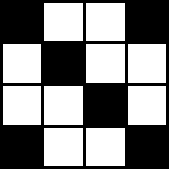
\includegraphics{images/ausfuell-1.pdf}
\qquad
\qquad
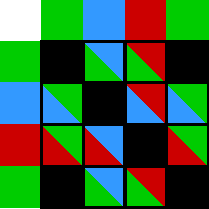
\includegraphics{images/ausfuell-2.pdf}
\caption{Ausfüllrätsel zum Grapheinfärbeproblem aus
Abbildung~\ref{vertex-coloring-examples}, links das leere `Spielfeld',
rechts ausgefüllt mit den Farben der Knoten.
\label{ausfuell:coloring}}
\end{figure}
Sehr viele Rätsel werden auf einem rechteckigen Feld von Zellen
bespielt, in die man etwas eintragen muss.
Sogar das Graphenfärbeproblem (\textsl{VERTEX-COLORING}) kann man
so auffassen.
Dazu formt man den gegebenen Graphen mit $n$ in eine
$n\times n$-Tabelle um, die Zeilen und Spalten entsprechen den Knoten
des Graphen, die Felder den möglichen Kanten.
Alle Felder, die zu im Graphen nicht existierenden Kanten gehören,
werden schwarz gefärbt.
In die weissen Felder müssen jetzt Paare von verschiedenen Farben
eingetragen werden, so dass in jeder Zeile die erste Farbe immer
gleich ist, und in jeder Spalte die zweite Farbe.
Ausserdem muss die Farbe einer Spalte und der entsprechenden Zeile
gleich sein.
Der Graph ist einffärbbar, wenn es möglich ist, die Tabelle wie
beschrieben auszufüllen (Abbildung~\ref{ausfuell:coloring}).

\begin{definition}
Ein {\em polynomielles Ausfüllrätsel} ist eine $n\times m$-Tabelle,
in die Zeichen eines Alphabets $\Sigma$ eingefüllt werden müssen,
so dass gewisse Regeln eingehalten werden.
Die einzuhaltenden Regeln können durch eine logische Formel beschrieben
werden, die in einer Zeit polynomiell in $nm$ berechnet werden kann.
\end{definition}

Die Bedingung der Berechenbarkeit in polynomieller Zeit ist meistens
offensichtlich.
Oft entsteht die Formel nämlich durch Anpassung der immer gleichen
Regeln für jedes Feld.
In solchen Fällen genügt es, wenn die resultierende Formel polynomielle
Länge hat.

\begin{beispiel}
Die Formel, die die Sudoku-Regeln für das $n^2\times n^2$-beschreibt,
besteht aus einer 
Teilformel für jedes Feld, welche wiederum aus einer Teilformel
für Zeilen, Spalten und Unterfelder besteht.
Diese Teilformeln überprüfen die Werte aller $n^2$ Felder der Zeile,
Spalte oder des Unterfeldes, dabei sind $n^2$ mögliche Feldinhalte
zu berücksichtigen.
Im Abschnitt~\ref{subsection:sudoku-und-sat} wurde gezeigt, wie die
Teilformel aufzubauen ist, ihre Länge ist
\[
O(\underbrace{n^2}_{\text{Vergleichsfelder}}\cdot
\underbrace{n^2}_{\text{Zeichen}}) = O(n^4).
\]
Die gesamte Formel hat damit die Länge
\[
O(\underbrace{n^4}_{\text{Felder}}\cdot
\underbrace{n^2}_{\text{Vergleichsfelder}}\cdot
\underbrace{n^2}_{\text{Zeichen}}) = O(n^8).
\]
Insbesondere ist die Länge der Formel polynomiell in der Feldgrösse $n^4$,
\textsl{SUDOKU}
ist also ein polynomielles Ausfüllrätsel im genannten Sinn.
\end{beispiel}

\begin{satz}
Ein polynomielles Ausfüllrätsel $A$ lässt sich polynomiell auf 
\textsl{SAT} reduzieren.
\end{satz}

\begin{proof}[Beweis]
Polynomielle Reduktion auf \textsl{SAT} bedeutet, dass man zu jeder
Probleminstanz eine logische Formel $\varphi$ konstruieren muss,
deren Länge polynomiell in der Grösse des Ausgangsproblems ist.
Die Formel muss genau dann erfüllbar sein, wenn das ursprüngliche
Problem lösbar ist.
Ein polynomielles Ausfüllrätsel führt aber nach Definition auf
eine solche Formel.
\end{proof}

Als Konsequenz dieser Konstruktion können wir auch schliessen, dass
jedes Ausfüllrätsel in NP liegt.



\subsection{Beweis des Satzes von Cook-Levin}

NP-vollständig heisst, dass jedes beliebige Problem in polynomieller
Zeit auf ein \textsl{SAT}-Problem reduziert werden kann.
Wir müssen
also einen Algorithmus angeben, mit dem aus einer Turingmachine
$M$ und einem Wort $w$
eine logische Formel $\varphi$ konstruiert werden kann, die genau
dann erfüllbar ist, wenn die Turingmaschine $M$ das Wort $w$
akzeptieren kann.

Die nicht deterministische Turingmaschine $M$ hat polynomielle Laufzeit,
jede Berechnung auf Inputwörter der Länge $n$ ist einer Zeit $n^k$
abgeschlossen. In dieser Zeit kann die Maschine höchstens $n^k$ Felder
des Bandes beschreiben, es wird also höchstens ein Abschnitt der
Länge $n^k$ des Bandes benutzt. Dabei werden maximal $n^k$
Konfigurationen durchlaufen. Schreibt man diese untereinander,
haben alle Konfigurationen in einem Quadrat $n^k\times n^k$
Platz.

Die Aufgabe ist jetzt also, das $n^k \times n^k$-Quadrat so mit Zuständen
und Symbolen auszufüllen, dass eine gültige Berechnung beschrieben wird,
die im Zustand $q_{\text{accept}}$ endet.
Dies ist ein Ausfüll-Rätsel, es bleibt uns also nur noch zu verstehen,
dass es sich auch um ein polynomielles Ausfüllrätsel handelt,
dass wir also die Bedingungen, denen die Symbole unterworfen sind,
in eine polynomielle Formel gefasst werden können.

Wir möchten jetzt also eine Formel aufstellen, die genau dann wahr
ist, wenn sich in das Quadrat $n^k\times n^k$ die Bandsymbole und
Zustände so hineinschreiben lassen, dass die Konfigurationen eine
Abfolge beschreiben, die einer gültigen Berechnung entsprechen.

Die einzelnen Zellen $c_{ij}$ der Tabelle sind mit einer Zeilennummer $i$
und einer Spaltennummer $j$ indiziert, in jede Zelle kann
genau ein Zeichen $z_{ij}$ geschrieben werden.
Zeichen können entweder Bandalphabetzeichen oder Zustände sein.
Der grösseren Einheitlichkeit wegen markieren wir die Enden des verwendeten
Bandabschnittes mit einem weiteren, bisher unbenutzten Zeichen {\tt\#}.
In einer Zelle finden wir also immer ein Zeichen aus $C=Q\cup \Gamma\cup\{\text{\tt\#}\}$.
Wir verwenden die logischen
Variablen $x_{ijs}$ mit $1\le i,j\le n^k$ und $s\in C$, die
genau dann wahr ist, wenn die Zelle $c_{ij}$ das Zeichen $s$ enthält.

Wir wissen bereits aus Satz~\ref{skript:satz:vergleichsformel}, dass wir
eine Vergleichsformel polynomiell in eine logische Formel umwandeln
können, es ist also nur noch nötig, die Bedingungen für das Ausfüllrätsel
als Vergleichsformel zu schrieben.

%In jede Zelle muss genau ein Zeichen geschrieben werden. Damit die Zelle
%$c_{ij}$ ein Zeichen enthält, muss mindestens eine der Variablen $x_{ijs}$
%wahr sein. Es dürfen aber keine zwei Zeichen einer Zelle zugeordnet sein,
%$x_{ijs}\wedge x_{ijt}$ für zwei verschiedenen Zeichen $s$ und $t$ darf
%also nicht wahr sein. Also muss jede Formel
%$\neg(x_{ijs}\wedge x_{ijt})=\overline{x_{ijs}}\vee\overline{x_{ijt}}$
%für zwei verschiedene Zeichen wahr sein, zusammen mit der
%Bedingung, dass ein Zeichen in der Zelle steht, erhalten wir
%für die Zellen $c_{ij}$ die Formel
%\[
%\varphi_{c_{ij}}=
%\biggl(\bigvee_{s\in C} x_{ijs}\biggr)\wedge
%\bigwedge_{\myatop{s,t\in C}{s\ne t}} (\overline{x_{ijs}}\vee\overline{x_{ijt}}).
%\]
%Dies muss für jede Indexkombination gelten, also
%\[
%\varphi_c
%=
%\bigwedge_{1\le i,j\le n^k}
%\varphi_{c_{ij}}
%=
%\bigwedge_{1\le i,j\le n^k}\biggl(
%\biggl(\bigvee_{s\in C} x_{ijs}\biggr)\wedge
%\bigwedge_{\myatop{s,t\in C}{s\ne t}} (\overline{x_{ijs}}\vee\overline{x_{ijt}})
%\biggr).
%\]
%Da unsere Redukton polynomiell sein soll, müssen wir auch bestimmen,
%wie lang die Formel $\varphi_c$ ist. Alle Formeln $\varphi_{c_{ij}}$
%sind gleich gross, abhängig nur von $|C|$, also einer Konstanten.
%Damit ist die Länge von $\varphi_c$ bestimmt durch die Grösse der
%Tabelle, also $O(n^2k)$. Die zum Aufbau von $\varphi_c$ notwendig Zeit
%ist ebenfalls $O(n^2k)$.

\subsubsection{Start mit dem Wort $w$}
Als nächstes drücken wir in einer Formel $\varphi_i$ aus,
dass die Turingmaschine mit dem
Wort $w$ initialisiert worden ist. Dazu muss in irgendeiner
Zelle der ersten Zeile das Zeichen $q_0$ stehen, und rechts
anschliessend die Zeichen des Wortes $w=a_1a_2\dots a_{|w|}$.
Steht $q_0$ in der
Zelle $j$, wird die Formel
\[
\varphi_{\text{start},j}
=
x_{11\#}\wedge
x_{12\blank}\wedge \dots \wedge
x_{1,j-1,\blank}\wedge
x_{1,j,q_0}\wedge
x_{1,j+1,a_1}\wedge\dots\wedge
x_{1,j+|w|,a_{|w|}}\wedge
x_{1,j+|w|+1,\blank}\wedge\dots\wedge
x_{1,n^k,\#}
\]
wahr.
Soll der Initialisierungsstring irgendwo in der ersten Zeile
stehen, wird eine der Formeln war, also
\[
\varphi_{\text{start}} = \bigvee_{1\le j\le n^k} \varphi_{\text{start}_j}.
\]
Auch diese Formel ist nicht grösser als $O(n^{2k})$ und kann in
polynomieller Zeit erzeugt werden.

\subsubsection{Akzeptierzustand}
Irgendwo in der Tabelle muss der Akzeptierzustand $q_\text{accept}$
stehen, also wir können dies durch 
\[
\varphi_{\text{accept}} 
=
\bigvee_{1\le i\le n^k} x_{N,i,q_{\text{accept}}}.
\]
ausdrücken.

\subsubsection{Berechnungsgeschichte}
Die Konfigurationen in der Tabelle müssen alle durch
Turingmaschinenübergänge auseinander hervorgehen, die Tabelle muss
mit einer Berechnungsgeschichte ausgefüllt werden.
Ob dies der Fall ist, kann durch die Betrachtung von zwei Zeilen
hohen und drei Zellen breiten Ausschnitten aus der Tabelle
überprüft werden.
Solche Ausschnitte zeigen fast immer zwei
gleiche Zeilen, ausser an der aktuellen Kopfposition, wo
sich etwas ändern kann.

Ein Übergang
\[
\entrymodifiers={++[o][F]}
\xymatrix{
p\ar[r]^{a\to b,R}
	&q
}
\]
wird zum Beispiel in den Ausschnitten
\[
\begin{tabular}{|c|c|c|}
\hline
$x$&$y$&$p$\\
\hline
$x$&$y$&$b$\\
\hline
\end{tabular}
\quad
\begin{tabular}{|c|c|c|}
\hline
$y$&$p$&$a$\\
\hline
$y$&$b$&$q$\\
\hline
\end{tabular}
\quad
\begin{tabular}{|c|c|c|}
\hline
$p$&$a$&$x$\\
\hline
$b$&$q$&$x$\\
\hline
\end{tabular}
\quad
\begin{tabular}{|c|c|c|}
\hline
$a$&$x$&$y$\\
\hline
$q$&$x$&$y$\\
\hline
\end{tabular}
\]
sichtbar. Ein Übergang mit einer Kopfbewegung nach links
\[
\entrymodifiers={++[o][F]}
\xymatrix{
p\ar[r]^{a\to b,L}
	&q
}
\]
dagegen in den Ausschnitten
\[
\begin{tabular}{|c|c|c|}
\hline
$z$&$x$&$y$\\
\hline
$z$&$x$&$q$\\
\hline
\end{tabular}
\quad
\begin{tabular}{|c|c|c|}
\hline
$x$&$y$&$p$\\
\hline
$x$&$q$&$y$\\
\hline
\end{tabular}
\quad
\begin{tabular}{|c|c|c|}
\hline
$y$&$p$&$a$\\
\hline
$q$&$y$&$b$\\
\hline
\end{tabular}
\quad
\begin{tabular}{|c|c|c|}
\hline
$p$&$a$&$x$\\
\hline
$y$&$b$&$x$\\
\hline
\end{tabular}
\quad
\begin{tabular}{|c|c|c|}
\hline
$a$&$x$&$y$\\
\hline
$b$&$x$&$y$\\
\hline
\end{tabular}
\]
Es gibt eine endliche Anzahl korrekter Belegungen solcher
$2\times 3$-Ausschnitte mit den Zeichen aus $C$, die Anzahl
hängt nur von $|C|$ und den Übergängen der Turingmaschine ab.

Jetzt müssen wir zeigen, dass wir gültige Übergänge, die durch erlaubte
Inhalte von $2\times 3$-Ausschnitten charakterisiert sind, mit
einer Vergleichsformel erkennen können.
Wir können aber für jede Ausschnitt-Position eine Vergleichsformel
aufstellen, die wahr wird, wenn die Zeichen im Ausschnitt 
gleich sind zu einem erlaubten Ausschnitt.
Insbesondere gibt es eine Vergleichsformel für Ausschnitt-Inhalte.

%Die Belegung
%\[
%\begin{tabular}{|c|c|c|}
%\hline
%$a_1$&$a_2$&$a_3$\\
%\hline
%$a_4$&$a_5$&$a_6$\\
%\hline
%\end{tabular}
%\]
%eines Ausschnitts mit der Zelle $c_{ij}$ in der
%linken oberen Ecke entspricht 
%\[
%x_{i,j,a_1}\wedge
%x_{i+1,j,a_2}\wedge
%x_{i+2,j,a_3}\wedge
%x_{i,j+1,a_4}\wedge
%x_{i+1,j+1,a_5}\wedge
%x_{i+2,j+1,a_6}.
%\]
%Davon muss eine wahr sein, also
%\[
%\varphi_{\text{Ausschnitt}_{ij}}
%=
%\bigvee_{\text{$a_1,\dots,a_6$ korrekt}}
%x_{i,j,a_1}\wedge
%x_{i+1,j,a_2}\wedge
%x_{i+2,j,a_3}\wedge
%x_{i,j+1,a_4}\wedge
%x_{i+1,j+1,a_5}\wedge
%x_{i+2,j+1,a_6}.
%\]
%Ausserdem muss jeder Ausschnitt gültig belegt sein, also
%muss
%\[
%\varphi_{\text{Ausschnitt}} =\bigwedge_{1\le i,j\le n^k}\varphi_{\text{Ausschnitt}_{ij}}
%\]
%wahr sein. Auch diese Formel lässt sich in polynomieller Zeit konstruieren
%und sie hat polynomielle Länge.

\subsubsection{Maschine hält auf einem Akzeptierzustand an}
Die Maschine kann schon wesentlich früher anhalten, also die worst case
Laufzeit anzeigt.
Wir müssen die Tabelle daher nach Ende der Berechnung mit immer gleichen
Zeilen ausfüllen.
Wir können dies erreichen, indem wir den erlaubten Ausschnitt-Inhalten
die drei Ausschnitte
\[
\begin{tabular}{|>{$}c<{$}|>{$}c<{$}|>{$}c<{$}|}
\hline
q_*&x&y\\
\hline
q_*&x&y\\
\hline
\end{tabular}
\qquad\text{oder}\qquad
\begin{tabular}{|>{$}c<{$}|>{$}c<{$}|>{$}c<{$}|}
\hline
x&q_*&y\\
\hline
x&q_*&y\\
\hline
\end{tabular}
\qquad\text{oder}\qquad
\begin{tabular}{|>{$}c<{$}|>{$}c<{$}|>{$}c<{$}|}
\hline
x&y&q_*\\
\hline
x&y&q_*\\
\hline
\end{tabular}
\]
mit $q_*\in\{q_\text{accept},q_\text{reject}\}$ und beliebigen
Bandalphabetzeichen $x$ und $y$ hinzufügen.

Wir haben also mehrere logische Formeln und Vergleichsformeln
gefunden, die genau dann alle wahr sind, wenn die Tabelle mit einer
akzeptierenden Berechnungsgeschichte gefüllt ist.
Die einzelnen Teile sind von polynomieller Grösse, also auch deren
Konjunktion.
Damit ist gezeigt, dass sich $A$ polynomiell auf ein polynomielles
Ausfüllrätsel reduzieren lässt.

%Damit die Tabelle eine akzeptierende Berechnung beschreibt, müssen
%alle Teile wahr sein, also ist
%\[
%\varphi =
%\varphi_{c}\wedge
%\varphi_{\text{start}}\wedge
%\varphi_{\text{accept}}\wedge
%\varphi_{\text{Ausschnitt}}
%\]
%die gesuchte Formel, die genau dann erfüllbar ist, wenn $w$ von der
%Turingmaschine $M$ akzeptiert werden kann.


%
% beispiele.tex -- Beispiele 
%
% (c) 2011 Prof Dr Andreas Mueller, Hochschule Rapperswil
%
\section{Beispiele NP-vollständiger Probleme}
\rhead{NP-vollständige Probleme}
Viele praktisch wichtige Probleme sind NP-vollständig. Der Nachweis
der NP-Vollständigkeit ist jedoch nicht immer einfach. Im Allgemeinen
wird er dadurch geführt, dass eine Reduktion von einem bereits als
NP-vollständig bekannten Problem konstruiert wird. Es lohnt sich
daher, einen möglichst grossen Katalog von NP-vollständigen
Problemen kennen zu lernen, einerseits um Übung im Konstruieren
von Reduktionen zu erhalten, andererseits um eine grössere Auswahl 
von Problemen zu bekommen, von denen ausgehend eine Reduktion 
konstruiert werden könnte. In diesem Kapitel werden einige
solche Probleme vollständig untersucht.
\subsection{3SAT}
\index{3SAT@\textsl{3SAT}}%
\begin{satz}
$\text{\textsl{3SAT}}$ ist NP-vollständig.
\end{satz}

\begin{proof}[Beweis]
Zum Beweis muss eine polynonmielle Reduktion
$\text{\textsl{SAT}}\le_P\text{\textsl{3SAT}}$ konstruiert werden.
Eine Reduktionsabbilung
$\text{\textsl{SAT}}\to\text{\textsl{3SAT}}$ muss eine allgemeine Formel
$\varphi$ in eine gleichwertige Formel in konjunktiver Normalform umwandeln, 
die ausserdem nur noch maximal drei Variablen in jeder Klausel enthält.

Ein erster Versuch verwendet die Distributivgesetze für die 
logischen Operationen, also
\begin{align*}
a\wedge(b\vee c)&=(a\wedge b)\vee(a\wedge c)\\
a\vee(b\wedge c)&=(a\vee b)\wedge(a\vee c),
\end{align*}
um die $\wedge$ nach ``aussen'' und die $\vee$ nach ``innen'' zu
bringen. Aus der Formel 
\begin{equation}
(x_1\wedge y_1)
\vee
(x_2\wedge y_2)
\vee
\dots
\vee
(x_n\wedge y_n)
\label{exponentialformula}
\end{equation}
wird, wie schon in (\ref{bigcnf}) bemerkt, eine Konjunktion von $2^n$
Termen der Form
\[
(u_1\vee u_2\vee \dots u_n)
\]
wobei $u_i=x_i$ oder $u_i=y_i$ sein kann. 
Die entstehende Konjunktion hat also exponentiell viele Terme, insbesondere
ist es nicht möglich, auf diesem Weg eine Reduktion
$f\colon\text{\textsl{3SAT}}\to\text{\textsl{SAT}}$ zu konstruieren.

Die gesuchte ``gleichwertige'' Formel muss nur im Sinne des
\textsl{SAT}-Problems gleichwertig sein, sie muss nicht eine
logisch äquivalente Formel sein. Es reicht, wenn die transformierte
Formel genau dann erfüllbar ist, wenn auch die ursprüngliche Formel
erfüllbar ist. Das bedeutet auch, dass wir neue Variablen einführen
dürfen.

Das Problem in Formel (\ref{exponentialformula}) entstand dadurch, dass
beim ``ausmultiplizieren'' sehr viele Kombinationen entstehen. Hätte
man eine Abkürzung $z_i=x_i\wedge y_i$, würde die Formel viel
kürzer, nämlich nur
\[
z_1\vee z_2\vee\dots\vee z_n.
\]
Diese Formel wäre sogar in konjunktiver Normalform, da man sie
als Formel mit nur einer Klausel betrachten kann.
Die Bedingung, dass man mit $z_i$ eigentlich $x_i\wedge y_i$ 
meint, kann man auch als 
\[
(x_i\wedge y_i)\Rightarrow z_i
=
z_i\vee \neg(x_i\wedge y_i)
=
z_i\vee \bar x_i\vee\bar y_i
\]
formulieren.
Die Übersetzung der Formel (\ref{exponentialformula})
in konjunktive Normalform ist dann
\begin{equation}
(z_1\vee z_2\vee\dots\vee z_n)
\wedge
\bigwedge_{i=1}^n (z_i\vee \bar x_i\vee\bar y_i).
\label{equivalentcnfformula}
\end{equation}
In (\ref{equivalentcnfformula}) kommen $4n$ Variablen vor,
in der ursprünglichen Formel
nur $2n$, die Formel wird also um den Faktor $2$ länger, die
Vergrösserung ist jetzt linear, nicht mehr exponentiell.

Es genügt also Regeln anzugeben, mit denen man Konjunktionen
``nach aussen'' bringen kann, so dass die Erfüllbarkeit der
Formel erhalten bleibt, und so dass die Länge der Formel 
höchstens polynomiell zunimmt. Für die Formel
\[
\varphi=
(
\varphi_{11}
\wedge
\varphi_{12}
\wedge
\dots
\wedge
\varphi_{1n_1}
)
\vee
(
\varphi_{21}
\wedge
\varphi_{22}
\wedge
\dots
\wedge
\varphi_{2n_2}
)
\vee\dots\vee
(
\varphi_{k1}
\wedge
\varphi_{k2}
\wedge
\dots
\wedge
\varphi_{kn_k}
)
\]
verwendet man wieder Variablen $z_i$, welche dafür die einzelnen
Klammerausdrücke stehen. Um auszudrücken, dass diese wahr sein
sollen, wenn die Klammerausdrücke wahr sind, fügt man
die Bedingungen
\[
z_i\vee \neg
(
\varphi_{i1}
\wedge
\varphi_{i2}
\wedge
\dots
\wedge
\varphi_{in_i}
)
=
z_i\vee
\neg\varphi_{i1}
\vee
\neg\varphi_{i2}
\vee
\dots
\vee
\neg\varphi_{in_i}
\]
hinzu. So erhält man die Formel
\[
(z_1\vee z_2\vee \dots\vee z_k)
\wedge
\bigwedge_{i=1}^k \biggl(z_i\vee \bigvee_{j=1}^{n_i} \neg\varphi_{ij}\biggr).
\]
Ihre Länge ist $O(k+\sum_{j=1}^k(1+n_j))=O(|\varphi|)$.
Durch wiederholte Anwendung dieser Methode kann die
Formel also in polynomieller Zeit in konjunktive Normalform gebracht
werden.

Die inzwischen erreichte konjunktive Normalform der Formel kann durchaus
noch mehrere Variablen pro Klausel enthalten. Sei 
\[
(x_1\vee x_2\vee \dots\vee x_n)
\]
eine solche Klausel.
Wir müssen sie ersetzen durch eine
Formel in konjunktiver Normalform mit drei Variablen pro Klausel.
Dazu kann man den folgenden Trick verwenden.
Die Formel $(\varphi\vee\psi)$ wird wahr, wenn eine der Unterformeln
$\varphi$ oder $\psi$ wahr ist. Sie wird nicht wahr sein, wenn 
beide Unterformeln nicht wahr sind. Sei $z$ eine neue Variable,
wir möchten mit ihr ausdrücken, dass $\psi$ wahr ist. Wir
verlangen $\bar z \vee \psi$, wenn $\psi$ nicht wahr ist, darf auch $z$
nicht wahr sein. Dann ist die Formel
\[
(\varphi \vee z)\wedge(\bar z\vee \psi)
\]
genau dann erfüllbar, wenn $\varphi\vee \psi$ erfüllbar ist.
Ist $\varphi$ nicht erfüllbar, dann muss $z$ wahr sein, und
damit auch $\varphi$, d.\,h.~auch $\varphi\vee\psi$ ist erfüllbar.
Eine zu lange Disjunktion kann also immer in kürzere Disjunktionen 
aufgespaltet werden. Rekursive Anwendung liefert jetzt eine Formel
mit maximal drei Literalen pro Klausel.
\end{proof}

\begin{satz}
$\text{\textsl{CLIQUE}}$ ist NP-vollständig.
\end{satz}

\begin{proof}[Beweis]
Da wir bereits früher gezeigt haben, dass
$\text{\textsl{3SAT}}\le_P\text{\textsl{CLIQUE}}$ ist, folgt jetzt auch,
dass $\text{\textsl{CLIQUE}}$ NP-vollständig ist.
\end{proof}

\subsection{Hamiltonscher Pfad}
Ein Hamiltonscher Pfad in einem gerichteten Graphen ist ein Pfad, der jeden
Vertex des Graphen genau einmal besucht. Als Sprachproblem formuliert 
\[
\text{\textsl{HAMPATH}}
=\{\langle G\rangle\,|\,\text{$G$ ist ein Graph mit einem hamiltonschen Pfad}\}
\]
Es ist leicht, zu verifizieren, ob
ein Pfad ein Hamiltonscher Pfad ist:
\begin{satz} $\text{\textsl{HAMPATH}}\in\text{NP}$.
\end{satz}

\begin{proof}[Beweis]
Als Zertifikat $c$ verwendet man den Pfad. Seine Länge ist geringer
als die Länge der Beschreibung des Graphen selbst.
Die Punkte des Pfades müssen benachbart sein, dies kann man in 
$O(n)$ testen.
Dann muss man überprüfen, ob jeder Vertex des Graphen vorkommt,
dies ist in Zeit $O(n^2)$ möglich. Auf dem Pfad darf kein Vertex
zweimal vorkommen, auch dies kann man in $O(n^2)$ verifizieren.
Insgesamt kann man also in polynomieller Zeit nachprüfen, ob ein
Pfad tatsächlich ein hamiltonscher Pfad ist.
\end{proof}

\begin{satz} \textsl{HAMPATH} ist NP-vollständig.
\end{satz}

\begin{proof}[Beweis]
Da bereits bekannt ist dass \textsl{HAMPATH} in NP ist, muss nur
noch eine Reduktion von einem bekanntermassen NP-vollständigen
Problem auf \textsl{HAMPATH} konstruiert werden. Die hier vorgestellte
ingeniöse Konstruktion reduziert \textsl{3SAT} auf \textsl{HAMPATH}.
Dazu muss zu jeder \textsl{3CNF}-Formel ein gerichteter Graph angegeben
werden, der genau dann einen hamiltonschen Pfad besitzt, wenn die
Formel erfüllbar ist.

Sei also $\varphi$ eine \textsl{3CNF}-Formel mit $k$ Klauseln in den Variablen
$x_1,\dots,x_n$. Der zu konstruierende Graph muss zu jeder Variablen
$x_i$ einen Teilgraphen enthalten, mit dem ausserdem ausgedrückt
werden kann, ob die Variable wahr oder falsch ist. Der Graph
\[
\entrymodifiers={++[o][F]}
\xymatrix{
*+\txt{}
	&*+\txt{}
		&*+\txt{}
			&*+\txt{}
				&{} \ar@/_10pt/[ddllll]\ar@/^10pt/[ddrrrr]
					&*+\txt{}
						&*+\txt{}
							&*+\txt{}
								&*+\txt{}
\\
*+\txt{}
\\
{}\ar@/^/[r] \ar@/_10pt/[ddrrrr]
	&{}\ar@/^/[r] \ar@/^/[l]
		&{}\ar@/^/[r] \ar@/^/[l]
			&{}\ar@/^/[r] \ar@/^/[l]
				&*+\txt{\dots}\ar@/^/[r] \ar@/^/[l]
					&{}\ar@/^/[r] \ar@/^/[l]
						&{}\ar@/^/[r] \ar@/^/[l]
							&{}\ar@/^/[r] \ar@/^/[l]
								&{} \ar@/^/[l]\ar@/^10pt/[ddllll]
\\	
*+\txt{}
\\
*+\txt{}
	&*+\txt{}
		&*+\txt{}
			&*+\txt{}
				&{}
					&*+\txt{}
						&*+\txt{}
							&*+\txt{}
								&*+\txt{}
}
\]
hat genau zwei hamiltonsche Pfade, die die ``Perlenkette'' in der
Mitte in entgegengesetzter Richtung durchlaufen.
Wir konstruieren einen Graphen, der
genau $n$ solche Teilgraphen untereinander enthält. Der $i$-te solche
Teilgraph steht für die Variable $x_i$. Der Durchlaufsinn der ``Perlenkette''
von links nach rechts bedeutet, dass diese Variable wahr sein soll,
der Durchlaufsinn von rechts nach links bedeutet, dass sie falsch ist.

Die Formel $\varphi$ besteht aus $k$ Klauseln, hat also die
Form $c_1\wedge c_2\wedge\dots\wedge c_k$. Wir wollen die Tatsache,
dass Klausel $c_j$ wahr ist, dadurch ausdrücken, dass der Pfad einen
Vertex $c_j$ besucht. $c_j$ kann von der Variablen $x_i$ wahr gemacht
werden wird dadurch ausgedrückt, dass der Pfad beim Durchlaufen
der ``Perlenkette'' von Variable $x_i$ einen ``Abstecher'' zu $c_j$
machen kann. Jedem Paar von Vertizes in der ``Perlenkette'' ordnen
wir daher eine Klausel zu. Falls $x_i$ in der Klausel $c_j$
vorkommte, fügen wir zwischen den beiden der Klausel $c_j$
zugeordneten Vertizes zusätzliche Kanten nach $c_j$ und wieder
zurück hinzu.
\[
\entrymodifiers={++[o][F]}
\xymatrix{
*+\txt{}
	&*+\txt{}
		&*+\txt{}
			&*+\txt{}
				&*+\txt{}
					&*+\txt{}
						&*+\txt{}
							&*+\txt{}
								&{c_j} \ar@/_15pt/[ddllll]
\\
*+\txt{}
	&*+\txt{}\ar[dl]
		&*+\txt{}
			&*+\txt{}
				&*+\txt{}
					&*+\txt{}
						&*+\txt{}\ar[dr]
							&*+\txt{} 
\\
{}\ar@/^/[r] \ar[dr]
	&{}\ar@/^/[r] \ar@/^/[l]
		&*+\txt{\dots}\ar@/^/[r] \ar@/^/[l]
			&{}\ar@/^/[r] \ar@/^/[l] \ar@/^15pt/[uurrrrr]
				&{}\ar@/^/[r] \ar@/^/[l]
					&*+\txt{\dots}\ar@/^/[r] \ar@/^/[l]
						&{}\ar@/^/[r] \ar@/^/[l]
							&{} \ar@/^/[l]\ar[dl]
\\
*+\txt{}
	&*+\txt{}
		&*+\txt{}
			&*+\txt{}
				\&*+\txt{}
					&*+\txt{}
						&*+\txt{}
							&*+\txt{}
}
\]
Enthält die Klausel $c_j$ die Variable $\bar x_i$ wird der
``Abstecher'' zu $c_j$ in die Durchlaufrichtung von rechts nach
links eingebaut.

Die Auswahl von Wahrheitswerten für die Variablen $x_i$ entspricht
der Entscheidung, in welcher Richtung die ``Perlenketten'' durchlaufen
werden. Die Formel ist offenbar genau dann erfüllbar, wenn ein
Abstecher zu jeder Klausel $c_j$ möglich ist, oder wenn es einen
hamiltoschen Pfad gibt.

Die Konstruktion erzeugt einen Graphen mit $O(nk)$ Vertizes,
ist also sicher in polynomialer Zeit durchführbar. Also ist
$\text{\textsl{3SAT}}\le_P\text{\textsl{HAMPATH}}$.
\end{proof}

\subsection{SUBSET-SUM}
\index{SUBSET-SUM@\textsl{SUBSET-SUM}}%
Das Problem \textsl{SUBSET-SUM} ist auch bekannt als das Rucksack-Problem.
Gegeben ist eine Menge $S$ von ganzen Zahlen, kann man darin eine
Teilmenge finden, die als Summe einen bestimmten Wert $t$ hat?
Als Sprache formuliert:
\[
\text{\textsl{SUBSET-SUM}}
=\left\{
\langle S,t\rangle\,\left|\,
\begin{minipage}{3truein}
$S$ eine Liste von ganzen Zahlen, in der es eine Teilliste
$T\subset S$ gibt mit
\[
\sum_{x\in T}x=t.
\]
\end{minipage}\right.
\right\}
\]
Der Name ``Rucksack''-Problem rührt daher, dass man sich 
die Zahlen aus $S$ als ``Grösse'' von Gegenständen vorstellt, und
wissen möchte, ob man einen Rucksack der Grösse $t$ exakt füllen
kann mit einer Teilmenge von Gegenständen aus $S$.

\begin{satz}\textsl{SUBSET-SUM} ist NP-vollständig
\end{satz}

\begin{proof}[Beweis]
Es ist ziemlich klar, dass $\text{\textsl{SUBSET-SUM}}\in\operatorname{NP}$,
es ist also nur noch eine Reduktion zu konstruieren, wir wählen
$\text{\textsl{3SAT}}\le_P\text{\textsl{SUBSET-SUM}}$.

Zu einer \textsl{3CNF}-Formel $\varphi$ mit Variablen $x_1,\dots,x_l$
muss eine Menge von Zahlen $S$ und eine Zahl $t$ gefunden werden,
die genau dann eine Teilmenge mit Summe $t$ hat, wenn $\varphi$
erfüllbar ist.

\begin{table}
\begin{center}
\begin{tabular}{|c|ccccc|}
\hline
Zahl&1&2&3&\dots&$l$\\
\hline
$y_1$&1&0&0&\dots&0\\
$z_1$&1&0&0&\dots&0\\
$y_2$& &1&0&\dots&0\\
$z_2$& &1&0&\dots&0\\
$y_3$& & &1&\dots&0\\
$z_3$& & &1&\dots&0\\
\vdots&& & &     & \\
$y_l$& & & &\dots&1\\
$z_l$& & & &\dots&1\\
\hline
$t$&1&1&1&\dots&1\\
\hline
\end{tabular}
\end{center}
\caption{Abbildung der Variablen $x_i$ und $\bar x_i$ in Zahlen
eines \textsl{SUBSET-SUM}-Problems\label{subsetsumnumbers}}
\end{table}

Wir konstruieren Zahlen $y_i$ und $z_i$, die jeweils ausdrücken
ob $x_i$ wahr oder falsch ist. Wir bauen die Zahlen in einer
Stellendarstellung zu einer später zu bestimmenden genügend
grossen Basis auf. Sofern die Zahlen nur wenige Stellen haben, die 
von $0$ verschieden sind, gibt es bei der Addition keinen Übertrag.
Die Zahlen $y_i$ und $z_i$ müssen so sein, dass nur jeweils eine
in der Summe auftreten kann. Dies erreichen wir, wenn wir
sie gemäss Tabelle \ref{subsetsumnumbers} wählen.
Die Auswahl einer Teilmenge mit Summe $t$ ist gleichbedeutend
mit der Wahl einer Belegung der Variablen $x_i$ mit Wahrheitswerten.
\begin{table}
\begin{center}
\begin{tabular}{|c|ccccc|cccc|}
\hline
Zahl&1&2&3&\dots&$l$&$c_1$&$c_2$&\dots&$c_k$\\
\hline
$y_1$&1&0&0&\dots&0&1&0&\dots&0\\
$z_1$&1&0&0&\dots&0&0&0&\dots&0\\
$y_2$& &1&0&\dots&0&0&1&\dots&0\\
$z_2$& &1&0&\dots&0&1&0&\dots&0\\
$y_3$& & &1&\dots&0&1&1&\dots&0\\
$z_3$& & &1&\dots&0&0&0&\dots&0\\
\vdots&& & &     & & & &     & \\
$y_l$& & & &     &1&0&1&\dots&1\\
$z_l$& & & &     &1&0&0&\dots&0\\
\hline
$g_1$& & & &     & &1&0&\dots&0\\
$h_1$& & & &     & &1&0&\dots&0\\
$g_2$& & & &     & & &1&\dots&0\\
$h_2$& & & &     & & &1&\dots&0\\
\vdots&& & &     & & & &     & \\
$g_k$& & & &     & & & &     &1\\
$h_k$& & & &     & & & &     &1\\
\hline
$t$  &1&1&1&\dots&1&3&3&\dots&3\\
\hline
\end{tabular}
\end{center}
\caption{Reduktion von \textsl{3SAT} auf
\textsl{SUBSET-SUM}\label{subsetsumtable}}
\end{table}

Jetzt muss noch codiert werden, in welchen Klauseln von $\varphi$ 
die Variablen $x_i$ auftreten. Dazu fügen wir der Tabelle für jede
Klausel $c_i$ eine weiter Spalte hinzu, und tragen eine $1$ ein
in der Zeile von $y_i$ wenn $x_i$ in der Klausel $c_j$ vorkommt.
Falls $\bar x_i$ in $c_j$ vorkommt tragen wir eine $1$ in der Zeile
von $z_i$ ein.

Die Formel ist erfüllbar, wenn es eine Belegung mit Wahrheitswerten
gibt, die jede Klausel wahr macht. Dabei können auch mehrere Literale
in einer Klausel war werden, die Summe der Spalte einer wahren Klausel kann
also Werte zwischen 1 und 3 annehmen. Da die Summe $t$ exakt erreicht
werden muss, führen wir für jede Klausel zusätzliche Zahlen $g_j$ und
$h_j$ hinzu, die in der Spalte der Klausel $c_j$ eine $1$ haben und sonst
nur $0$. Indem man zur Teilmenge falls nötig $g_j$ und $h_j$ hinzunimmt,
kann man erreichen, dass die Summe in der Spalte von Klausel $c_j$ immer
$3$ ergibt.
Die Tabelle \ref{subsetsumtable} zeigt die konstruierten Zahlen
für die Formel
\[
(x_1\vee \bar x_2\vee x_3)\wedge(x_2\vee x_3\vee x_l)\wedge \dots\wedge
(\dots\vee \bar x_3).
\]
Da die grösste vorkommende Ziffer eine $3$ ist, kann man die
Zahlen aus $S$  und $t$ im $4$-er-System aus der Tabelle ablesen.

Der Zeitaufwand für die Erstellung der Tabelle \ref{subsetsumtable}
ist $O((k+l)^2)$, also sicher polynomiell in der Länge der
Formel $\varphi$.

Damit ist 
$\text{\textsl{3SAT}}\le_P\text{\textsl{SUBSET-SUM}}$ gezeigt.
\end{proof}

%\subsection{Vertex Coloring}
%Das Eckenfärbeproblem wurde bereits verwendet und seine Äquivalenz
%mit dem Stundenplanproblem gezeigt. Es ist auch einfach zu verifizieren,
%dass \textsl{VERTEX-COLORING} in NP ist. Daher ist es nicht überraschend,
%dass es auch NP-vollständig ist.
%
%\begin{satz}
%$\text{\textsl{3SAT}}\le_P\text{\textsl{VERTEX-COLORING}}$,
%insbesondere ist \textsl{VERTEX-COLORING} NP-vollständig.
%\end{satz}
%
%\begin{proof}[Beweis]
%Eine Reduktion
%$\text{\textsl{3SAT}}\le_P\text{\textsl{VERTEX-COLORING}}$
%ordnet einer \textsl{3CNF}-Formel $\varphi$ einen Graphen $G$
%und eine Zahl $k$ zu, der genau dann mit $k$ Farben eingefärbt
%werden kann, wenn $\varphi$ erfüllbar ist.
%
%Wir verwenden $k=2$, die Bedeutung der zwei Farben soll wahr
%oder falsch sein. Die Formel $\varphi$ besteht aus $l$ verschiedenen
%Klauseln, wir schreiben 
%\[
%\varphi = c_1\wedge c_1\wedge \dots\wedge c_l.
%\]
%Dem Graphen $G$ fügen wir einen Knoten für jede Klausel hinzu,
%sowie einen Knoten $o$. Jede Klausel wird mit dem Knoten $o$ verbunden.
%Eine Einfärbung bedeutet, dass alle Klauseln mit der gleichen Farbe
%eingefärbt werden müssen, dies interpretieren wir als Ausdruck
%der Tatsache, dass in einer erfüllbaren Formel die Wahrheitswerte
%so gewählt werden können, dass alle Klauseln wahr werden.
%\[
%\xymatrix{
%*+\txt{}
%	&*+\txt{}
%		&*+[o][F-]{o}\ar@{-}[dll] \ar@{-}[dl] \ar@{-}[d] \ar@{-}[drr]
%\\
%*+[o][F-]{c_1}
%	&*+[o][F-]{c_2}
%		&*+[o][F-]{c_3}
%			&\dots
%				&*+[o][F-]{c_l}
%}
%\]
%
%Die Klauseln sind alle von der Form
%\[
%c_i=(x_1\vee x_2\vee x_3)
%=\neg(\bar x_1\wedge \bar x_2 \wedge \bar x_3).
%\]
%Damit sie wahr wird, muss $\bar x_1\wedeg \bar x_2\wedge \bar x_3$
%falsch sein.
%\end{proof}


%
% katalog.tex -- Katalog NP-vollständiger Probleme
%
% (c) 2011 Prof Dr Andreas Mueller, Hochschule Rapperswil
%
\section{Katalog NP-vollständiger Probleme von Karp}
\rhead{Liste von Karp}
\index{Karp, Richard}%
\index{Karp's Liste}%
Schon kurz nach der Veröffentlichung des Beweises des Satzes
\ref{cooklevin} hat Richard Karp einen Baum von Reduktionen
veröffentlicht, in dem ausgehend von SAT 21 Probleme verzeichnet
waren.
Selbstverständlich lässt
sich jedes dieser Probleme auf jedes andere reduzieren. Zum Beispiel
hatten wir \textsl{3SAT} auf \textsl{CLIQUE} reduziert, während
Karp direkt von \textsl{SAT} ausgeht. Karps Reduktionsbaum
beginnt wie folgt.
\[
\xymatrix{
{}
	&\text{\textsl{SAT}} \ar[dl] \ar[d] \ar[dr]
\\
\text{\textsl{CLIQUE}} \ar[d] \ar[dr]
	&\text{\textsl{BIP}}
		&\text{\textsl{3SAT}} \ar[d]
\\
\text{\textsl{VERTEX-COVER}}
	&\text{\textsl{SET-PACKING}}
		&\text{\textsl{VERTEX-COLORING}}
}
\]
Weiter oben haben wir \textsl{CLIQUE} von \textsl{3SAT} aus
reduziert. \textsl{VERTEX-COLORING} haben wir im Zusammenhang
mit dem Stundenplanproblem getroffen.

\index{BIP@\textsl{BIP}}%
\textsl{BIP} ist ``binary integer programming'', zu einer ganzzahligen
Matrix $C$ und einem ganzzahligen Vektor $d$ ist ein binärer
Vektor $x$ zu finden mit $Cx=d$.

\begin{satz}
\textsl{BIP} ist NP-vollständig.
\end{satz}

\begin{proof}[Beweis]
Es ist klar, dass \textsl{BIP} in NP ist. Es genügt daher, eine
Reduktion
\[
\text{\textsl{SUBSET-SUM}}\le_P\text{\textsl{BIP}}
\]
zu konstruieren.

Dazu muss zu einer Menge $S$ von ganzen Zahlen und einer Summe $t$
eine Matrix und ein Vektor konstruiert werden. Als Matrix nehmen wir
eine Matrix mit einer Zeile, in der die Elemente von $S$ stehen. Als
Vektor $d$ nehmen wir den Vektor mit der einen Komponenten $t$.
Einen binären Vektor $x$ finden mit $Cx=d$ ist jetzt gleichbedeutend
damit, eine Auswahl von Zahlen in $S$ zu finden, deren Summe $t$ ist.
Also ist
$\text{\textsl{SUBSET-SUM}}\le_P\text{\textsl{BIP}}$.
\end{proof}

Im folgenden wollen die von Karp als NP-vollständig erkannten Probleme
ohne Beweis im Sinne einer Referenz zusammenstellen. Hat man ein
Problem als NP-vollständig nachzuweisen, kann man von jedem dieser
Probleme aus eine Reduktion versuchen.

Für die Abhängigkeiten unterhalb von \textsl{VERTEX-COVER} gibt 
Karp folgenden Baum
\[
\xymatrix{
	&\text{\textsl{VERTEX-COVER}} \ar[dl] \ar[d]\ar[dr]\ar[drr]
\\
\begin{minipage}{1.0truein}
\textsl{FEEDBACK-NODE-SET}
\end{minipage}
	&\begin{minipage}{1.0truein}\textsl{FEEDBACK-ARC-SET}\end{minipage}
		&\text{\textsl{HAMPATH}}\ar[d]
			&\text{\textsl{SET-COVERING}}
\\
	&
		&\text{\textsl{UHAMPATH}}
}
\]
\textsl{UHAMPATH} ist das Problem in einem ungerichteten Graphen
einen hamiltonschen Pfad zu finden. Die anderen Probleme sind wie
folgt definiert:
\begin{description}
\index{VERTEX-COVER@\textsl{VERTEX-COVER}}%
\item[\textsl{VERTEX-COVER}:] Gegeben ein Graph $G$ und eine Zahl
$k$, gibt es eine Teilmenge von $k$ Vertizes so, dass jede
Kante des Graphen ein Ende in dieser Teilmenge hat?
\index{FEEDBACK-NODE-SET@\textsl{FEEDBACK-NODE-SET}}%
\item[\textsl{FEEDBACK-NODE-SET}:] Gegeben ein gerichteter Graph $G$
und eine Zahl $k$, gibt es eine endliche Teilmenge von $k$ Vertizes
von $G$ so, dass jeder Zyklus in $G$ einen Vertex in der Teilmenge 
enthält?
\index{FEEDBACK-ARC-SET@\textsl{FEEDBACK-ARC-SET}}%
\item[\textsl{FEEDBACK-ARC-SET}:] Gegeben ein gerichteter Graph $G$
und eine Zahl $k$, gibt es eine Teilmenge von $k$ Kanten so, dass
jeder Zyklus in $G$ eine Kante aus der Teilmenge enthält?
\index{SET-COVERING@\textsl{SET-COVERING}}%
\item[\textsl{SET-COVERING}:] Gegeben eine endliche Familie endlicher
Mengen $(S_j)_{1\le j\le n}$ und eine Zahl $k$, gibt es eine Unterfamilie
bestehend aus $k$ Mengen, die die gleiche Vereinigung hat?
\end{description}
Die Abhängigkeiten unter \textsl{VERTEX-COLORING} sind etwas vielfältiger:
\[
\xymatrix{
	&\begin{minipage}{1truein}
	\textsl{VERTEX-COLORING}
	\end{minipage} \ar[d]\ar[dr]
\\
	&\begin{minipage}{0.6truein}
	\textsl{EXACT-COVER}
	\end{minipage} \ar[dl] \ar[d] \ar[dr] \ar[drr]
		&\begin{minipage}{0.8truein}
		\textsl{CLIQUE-COVER}
		\end{minipage} 
\\
\text{\textsl{3D-MATCHING}}
	&\text{\textsl{SUBSET-SUM}} \ar[dr] \ar[d]
		&\begin{minipage}{0.8truein}
		\textsl{HITTING-SET}
		\end{minipage}
			&\begin{minipage}{0.8truein}
			\textsl{STEINER-TREE}
			\end{minipage}
\\
	&\text{\textsl{SEQUENCING}}
		&\text{\textsl{PARTITION}} \ar[d]
\\
	&
		&\text{\textsl{MAX-CUT}}
}
\]
\begin{description}
\item[\textsl{EXACT-COVER}] Gegeben eine Familie $(S_j)_{1\le j\le n}$
von Teilmengen
einer Menge $U$ gibt es eine Unterfamilie von Mengen, die disjunkt sind,
aber die gleiche Vereinigung haben?
Die Unterfamilie $(S_{j_i})_{1\le i\le m}$ muss also
$S_{j_i}\cap S_{j_k}=\emptyset$ und 
\[
\bigcup_{j=1}^n S_j=\bigcup_{i=1}^mS_{j_i}
\]
erfüllen.
\index{CLIQUE-COVER@\textsl{CLIQUE-COVER}}%
\item[\textsl{CLIQUE-COVER}:] Gegeben ein Graph $G$ und eine positive Zahl
$k$, gibt es $k$ Cliquen so, dass jede Ecke in genau einer der Cliquen ist?
\index{3D-MATCHING@\textsl{3D-MATCHING}}%
\item[\textsl{3D-MATCHING}:] Sei $T$ eine endliche Menge und $U$ eine 
Menge von Tripeln aus $T$: $U\subset T\times T\times T$.
Gibt es eine
Teilmenge $W\subset U$ so, dass $|W|=|T|$ und keine zwei Elemente
von $W$ stimmen in irgendeiner Koordinate überein?
\index{HITTING-SET@\textsl{HITTING-SET}}%
\item[\textsl{HITTING-SET}:] Gegeben eine Menge von Teilmengen $S_i\subset S$,
gibt es eine Menge $H$, die jede Menge in genau einem Punkt trifft, also
$|H\cap S_i|=1\forall i$?
\index{STEINER-TREE@\textsl{STEINER-TREE}}%
\item[\textsl{STEINER-TREE}:]
Gegeben ein Graph $G$, eine Teilmenge $R$ von Vertizes, und eine
Gewichtsfunktion $w\colon E\to\mathbb Z$ und eine postive Zahl $k$, gibt es
einen Baum mit Gewicht $\le k$, dessen Knoten in $R$ enthalten sind?
Das Gewicht des Baumes ist die Summe der Gewichte 
$w(\{u,v\})$ über alle Kanten $\{u,v\}$ im Baum.
\index{SEQUENCING@\textsl{SEQUENCING}}%
\item[\textsl{SEQUENCING}:] Gegeben sei ein Vektor
$(t_1,\dots,t_p)\in\mathbb Z^p$
von Laufzeiten von $p$ Jobs, ein Vektor von spätesten Ausführungszeiten 
$(d_1,\dots,d_p)\in\mathbb Z^p$, einem Strafenvektor 
$(s_1,\dots,s_p)\in\mathbb Z^p$ und eine positive ganze Zahl $k$.
Gibt es eine Permutation $\pi$ der Zahlen $1,\dots,p$, so dass
die Gesamtstrafe für verspätete Ausführung bei der Ausführung der Jobs
in der Reihenfolge $\pi(1),\dots,\pi(p)$ nicht grösser ist als $k$? 
Formal lautet die Bedingung
\[
\sum_{j=1}^p
\vartheta(t_{\pi(1)} +\dots +t_{\pi(j)} - d_{\pi(j)}) s_{\pi(j)} \le k,
\]
darin ist $\vartheta$ die Stufenfunktion definiert durch
\[
\vartheta(x)=\begin{cases}
1&x\ge 0\\
0&x<0.
\end{cases}
\]
\index{PARTITION@\textsl{PARTITION}}%
\item[\textsl{PARTITION}:] Gegeben ein Folge von $s$ ganzen Zahlen
$c_1,c_2,\dots,c_s$, kann man die Indizes $1,2,\dots,s$ in zwei
Teilmengen $I$ und $\bar I$ teilen, so dass die Summe der zugehörigen
$c_i$ identisch ist:
\[
\sum_{i\in I}c_i=\sum_{i\not\in I}c_i
\]
\index{MAX-CUT@\textsl{MAX-CUT}}%
\item[\textsl{MAX-CUT}:] Gegeben ein Graph $G$ mit einer Gewichtsfunktion
$w\colon E\to\mathbb Z$ und eine ganze Zahl $W$.
Gibt es eine Teilmenge
$S$ der Vertizes, so dass das Gesamtgewicht der Kanten, die $S$ mit
seinem Komplement verbinden, mindestens so gross ist wie $W$:
\[
\sum_{\{u,v\}\in E\wedge u\in S\wedge v\not\in S} w(\{u,v\})\ge W
\]
\index{SET-PACKING@\textsl{SET-PACKING}}%
\item[\textsl{SET-PACKING}:] Gegeben eine Familie $(S_i)_{i\in I}$ von
Mengen und eine Zahl $k\in \mathbb N$.
Gibt es eine $k$-elementige Teilfamilie $(S_i)_{i\in J}$ mit $J\subset I$,
d.~h.~$|J|=k$,
derart,
dass die Mengen der Teilfamilie paarweise diskjunkt sind, also 
\[
	S_i \cap S_j = \emptyset \quad\forall i,j\in J \;\text{mit}\; i\ne j?
\]
\end{description}



%
% karp.tex -- Beispiele zum Katalog von Karp
%
% (c) 2019 Prof Dr Andreas Müller, Hochschule Rapperswil
%
\section{Beispiele}
\rhead{Beispiele zur Liste von Karp}
In diesem Abschnitt werden zu den NP-vollständigen Problemen des
Katalogs von Karp einzelne Beispiele oder Illustrationen geben.
\subsection{VERTEX-COVER}
Diktator Revoc Xetrev unterdrückt sein Volk gnadenlos.
Schon länger lässt er von der staatlichen Telefongesellschaft
erheben, welche Telefonanschlüsse genau miteinander telefonieren.
Damit lassen sich hervorragend Leute als Regimefeinde entlarven.
Nachdem allerdings eine ganze Reihe von hohen Militärs als
Landesverräter verurteilt und erschossen worden waren,
stellte sich heraus, dass eine Gruppe von
inzwischen ebenfalls verurteilten Regimekritikern sich genau dies
zu Nutze machten: sie riefen die Militärs gegen deren Willen an.
Da es keine Aufzeichnung über den Inhalt der Gespräche gab, konnten
die Militärs ihre Unschuld nicht beweisen, mit fatalen Folgen für
ihre Karriere.

Diese Affäre hatte das Militär einige der fähigsten Köpfe beraubt,
so dass eine zuverlässigere Methode gefunden werden musste, um
Regimefeinde zu erkennen.
Wenn sich damit gegenüber dem Ausland auch noch ein Anschein von
Rechtssystem etablieren liess, würde das Diktator Xetrev den Zugang
zu westlichen Waffenlieferanten etwas erleichtern.

Aus technischen Gründen ist eine lückenlose Überwachung aller Anschlüsse
nicht möglich.
Die Software kann mit maximal $k$ Anschlüssen umgehen, die abgehört
werden können.
Diktator Xetrev befiehlt daher, dass innert einer Woche eine Menge
von $k$ Anschlüssen definiert werden müsse, so dass jedes
Telefongespräch abgehört werden kann.

Diese Ankündigung verursacht erst einmal eine neue Fluchtwelle von
Mathematikern und Informatikern.
Nach einer Woche wird der erste Experte wegen Befehlsverweigerung
erschossen.
Im Prozess, der nur 15 Minuten gedauert hatte, hatte er feige behauptet,
es sei nicht möglich, in der kurzen
Zeit eine entsprechende Menge zu finden.
Ja es sei nicht einmal
möglich, zu entscheiden, ob es eine solche Menge überhaupt gäbe.
Der Staatsanwalt legte ihm das als Sabotage der Pläne des grossen
Diktators Xetrev aus und machte kurzen Prozess mit ihm.

Als aber nach einer weiteren Woche erneut ein Saboteur angeklagt wurde,
der genau die gleiche Verteidigungstrategie verwendete, obwohl
doch mittlerweile bekannt war, dass sie nicht zum Erfolg führen konnte,
begann sich Diktator Xetrev zu fragen, ob darin vielleicht
ein Körnchen Wahrheit stecken könnte.
Könnte es sein, dass 
es tatsächlich zu schwierig ist, eine solche Anschlussauswahl zu treffen?

\medskip

Das Problem, welches die Experten lösen sollten, ist das Problem
{\it VERTEX-COVER}.
Die Telefonanschlüsse bilden die Knoten eines Graphen,
die Kanten verbinden diejenigen Anschlüsse, die tatsächlich miteinander
telefonieren.
Gesucht ist eine Menge von $k$ Knoten so, dass jedes
mögliche Gespräch abgehört werden kann, also jede Kante in einem
ausgewählten Knoten endet.


\subsection{FEEDBACK-NODE-SET}
In einer grossen Fabrik bringen Transportroboter die Teile zu den
Verarbeitungsstationen.
Die Roboter fahren dabei entlang vorgegebener
Bahnen, die sie mit Hilfe von Bodenmarkierungen einhalten.
Die Roboter
sind immer für die gleichen Prozesse im Einsatz und fahren daher mehrmals
am Tag immer die gleichen Runden ab.

Die Wartungsvorschriften verlangen, dass die Roboter täglich einmal einem
Sicherheitscheck unterzogen werden, der nur wenige Minuten dauert.
Wegen
des weitläufigen Fabrikgeländes lohnt es sich nicht, alle Roboter jeden
Tag an eine zentrale Kontrollstelle zu fahren, wo sie überprüft werden
können.
Sie würden viel zu lange ausfallen.
Daher wurde entschieden, an
einigen Knoten des Netzes der Roboter-Fahrwege Prüfstellen einzurichten.

Sachbearbeiter Heiri Muster soll herausfinden, ob das Budget reicht,
um genügend Prüfstellen einzurichten, so dass jeder Roboter täglich
geprüft werden kann.
Drei Monate später wird er wegen Burnout freigestellt.

\medskip

Das Budget reicht für die Ausrüstung von $k$ Prüfstellen.
Die Roboter bewegen sich auf dem gerichteten Graphen der Bodenmarkierungen.
Sie fahren die Zyklen des Graphen ab.
Gesucht wird jetzt eine Menge
von $k$ Netzknoten für die Prüfstellen, so dass jeder Zyklus des Graphen
durch eine dieser Prüfstellen verläuft.
Dies ist das NP-vollständige Problem {\it FEEDBACK-NODE-SET}.
Nach aktuellem Wissen gibt es keinen Algorithmus mit polynomieller
Laufzeit, der entscheiden könnte, ob das Problem überhaupt eine
Lösung hat.

\subsection{FEEDBACK-ARC-SET}
Kurz nachdem die Pläne für das Prüfstellennetz aus dem vorangegangenen
Beispiel von der Geschäftsleitung bewilligt worden waren, änderte
der Hersteller der Roboter bei einem Softwareupdate die Wartungsvorschriften.
Die Prüfung erfolgt jetzt nicht mehr im Stehen, sondern während der
Fahrt.
Durch diese dynamische Prüfung werden Probleme erkennbar, die bei der
statischen Prüfung nicht gefunden werden konnten.
Heiri Musters
Nachfolger wird beauftragt, die Pläne entsprechend anzupassen.
Drei Monate später ist auch er wegen Burnout freigestellt.

\medskip

Das Problem wurde durch die Umstellung zu einer Instanz des
Problems {\it FEEDBACK-ARC-SET} modifiziert.
Es müssen $k$ Kanten gefunden werden, so dass jeder Zyklus eine
diese Kanten durchläuft.
Auch dieses Problem ist NP-vollständig,
und dürfte daher für ein kompliziertes Streckennetz
nicht nur einen Sachbearbeiter überfordern.

\subsection{SET-COVERING}
Der populistische Politiker Tesco Vering versprach während des
Wahlkampfes, das Dickicht von Steuererleichterungen, welches
für jeden Bürger das Ausfüllen der Steuererklärung zur Qual
machte, zu vereinfachen.
Nach seinem Amtsantritt als Ministerpräsident 
stellte er jedoch fest, dass jeder seiner Wähler von irgendeiner
der Vergünstigungen profitierte.
Um seine Wiederwahl nicht
zu gefährden, beauftragte er daher eine Komission eine Liste
von Vergünstigungen aufzustellen, so dass jeder seiner Wähler
immer noch von einer Vergünstigung profitiert.
Niemand soll im
Wahlkampf sagen können: ``Vering hat mir alle Vergünstigungen weggenommen!''
Kurz vor Beginn des nächsten Wahlkampfs war die Komission jedoch
immer noch nicht fertig, so dass sich Vering als neues Wahlkampfthema
auf den Kampf gegen die allgemeine Unfähigkeit der Verwaltung verlegte,
um davon
abzulenken, dass er das letzte Wahlversprechen nicht eingelöst hatte.
Trotzdem wurde er nicht wiedergewählt.
Eine detaillierte Analyse der
Wahlresultate ergab, dass Vering vor allem die Stimmen der Mathematiker und
Informatiker gefehlt hatten.
Sie warfen ihm Unverständnis für die Komplexität seiner Aufgabe vor und 
hielten ihn deshalb für nicht tauglich für ein politisches Amt.

\medskip

Tatsächlich ist das Programm von Tesco Vering das Problem {\it SET-COVERING}.
Die Steuervergünstigungen sind numeriert von $1$ bis $n$.
Sei $S_i$ die Menge der Wähler von Vering, die von Vergünstigung $i$
profitieren.
Der Auftrag der Komission war, eine Teilmenge
$I=\{i_1,i_2,\dots,i_k\}$ zu finden, so dass
\[
\bigcup_{i=1}^nS_i=\bigcup_{i\in I}S_i
\]
ist.
Dieses Problem ist NP-vollständig, nach aktuellem Wissen gibt
es also keinen polynomiellen Algorithmus um zu entscheiden, ob es
überhaupt eine Lösung des Problems gibt.

\subsection{EXACT-COVER}
In einem Straflager müssen Sträflinge in diversen Bauprojekten
der Umgebung arbeiten.
Viele der Sträflinge sind jedoch eher unbegabt und daher kaum
fähig, diese Arbeiten zur Zufriedenheit der Lagerleitung auszuführen.
Jeder Sträfling ist für mindestens eines der Projekte nicht geeignet.
Der sadistische Lagerkommandant ersinnt sich dazu noch einen teuflischen
Plan, wie er möglichst viele Sträflinge wegen Sabotage bestrafen kann.
Er gibt seinen Schergen folgende Regeln für die Zuteilung der Sträflinge
zu den Projekten:
\begin{enumerate}
\item
An jedem Tag soll nur an einem Teil der Projekte gearbeitet werden.
\item
Alle für das Projekt ungeeigneten Sträflinge arbeiten an diesem Tag
an dem Projekt.
\item
Trotzdem muss eindeutig bestimmt sein, an welchem Projekt ein Sträfling
arbeiten soll.
\item
Jeder Sträfling muss eingesetzt sein.
\end{enumerate}
Im Lagerapport am nächsten Tag rücken die Aufseher damit heraus, dass
sie keine Zuteilung gefunden hätten, die diesen Regeln entspricht, und
dass deshalb an diesem Tag nichts gearbeitet worden sei.
Der Lagerkommandant schäumt vor Wut und droht damit die Aufseher eigenhändig
zu erschiessen, wenn sie sich weiterhin seinen Befehlen widersetzen
würden.

\medskip

Der Lagerkommandant hat seinen Aufsehern ein Problem gestellt, welches
äquivalent zu {\it EXACT-COVER} ist.
Die Menge aller Sträflinge ist $U$.
Die Projekte seien numeriert
von $1$ bis $n$.
Die Menge $S_i\subset U$ besteht aus den Sträflingen, die
für das Projekt $i$ ungeeignet sind.
Weil jeder Sträfling für mindestens
ein Projekt ungeeignet ist, ist 
\[
U=\bigcup_{i=1}^n S_i.
\]
Gesucht wird jetzt eine Teilmenge von Projekten
$I=\{i_1,\dots,i_m\}\subset\{1,\dots,n\}$, so dass 
jeder Sträfling auf einem Projekt arbeitet:
\[
\bigcup_{j=1}^m S_{i_j}=U
\]
aber kein Sträfling mehr als einem Projekt zugeteilt wird:
\[
S_{i_j}\cap S_{i_k}=\emptyset\qquad \forall j\ne k.
\]
Dieses Problem ist NP-vollständig, nach aktuellem Wissen gibt es
also keinen polynomiellen Algorithmus, mit dem entschieden werden
könnte, ob es überhaupt eine Lösung hat.

\subsection{CLIQUE-COVER}
Ein Beispiel für das CLIQUE-COVER-Problem ist die Aufgabe 7.11 in der
Aufgabensammlung.

\subsubsection{Abgeschwächtes CLIQUE-COVER}
Es gibt auch eine abgeschwächte Form des CLIQUE-COVER-Problems, wo
nicht verlangt wird, dass die Cliquen disjunkt sind.
Wir könnten dieses Problem WEAK-CLIQUE-COVER nennen.
Ein Beispiel für dieses abgeschwächte Problem könnte das folgende sein.

\medskip

In einem Online-Spiel treten die Spieler jeweils paarweise gegeneinander an.
Eine zuverlässige Rangliste der Spieler kann nur innerhalb
einer Gruppe erstellt werden, in der jeder Spieler gegen
jeden anderen gespielt hat.
Trotzdem soll jetzt versucht werden,
ein Gesamt-Ranking zu erstellen.
Grundlage dafür ist die Auswahl
einer Menge von Gruppen, in der jeder gegen jeden gespielt hat.
Die Auswahl soll möglichst klein sein, denn man hofft so, die
Schnittmengen, in denen systembedingt am ehesten Ranking-Widersprüche
auftreten könnten, möglichst klein zu halten.
Allerdings stellt es
sich als schwierig heraus, eine solche Auswahl zu treffen, warum?

\medskip

Die Aufgabe verlangt, in dem Graphen bestehend aus den Spielern
als Knoten und Kanten, die angeben, ob die zwei Spieler schon gegeneinander
gespielt hat, eine Überdeckung mit einer möglichst
kleinen Anzahl Cliquen zu finden.
Dies ist das NP-vollständige Problem {\it WEAK-CLIQUE-COVER}.
Nach aktuellem Wissen gibt es dafür keinen
Algorithmus mit polynomieller Laufzeit.

\subsection{3D-MATCHING}
In der Provinz Gnichtam De herrscht grosse Wohnungsnot.
Eine Analyse durch das Innenministerium ergab, dass die Ursache
die vielen Singles sind, die jeweils alleine eine gemäss
Plan der staatlichen Wohnungsbaubehörde für Familien vorgesehene
Wohnung belegen.
Würde man die Singles paarweise den Wohnungen zuteilen, würden die
Wohnungen reichen.

Daher beschliesst der Familienminister ein Programm zur Zwangsverheiratung
der Singles und beautragt seine Behörde mit der Ausarbeitung einer Zuordnung,
wer mit wem verheiratet werden soll und wo das frisch verheiratete Paar
wohnen soll.
Natürlich ist nicht jede Kombination aus einem Mann,
einer Frau und einer Wohnung akzeptabel, immerhin müssen 
Arbeitswege vernünftig bleiben, die Bürger sollen ja als 
Arbeiter weiterhin produktiv bleiben um die hohen Steuern bezahlen zu können.
Das Ministerium beginnt also eine Liste von möglichen Zwangsfamilien
zu erstellen.

Nach einem Jahr wird der Familienminister ungeduldig, denn obwohl die
genannte Liste nach wenigen Wochen fertig war, konnte daraus immer noch
keine geeignete Familienplanung abgeleitet werden, die Fachleute wissen
noch nicht einmal, ob es überhaupt möglich ist, eine Planung
zu finden, welche alle geforderten Rahmenbedingungen erfüllt.

\medskip

Das Problem, welches das Familienministerium der Provinz Gnichtam De
lösen soll, ist {\it 3D-MATCHING}.
Es gibt $n$ unverheiratete Frauen
und Männer, und $n$ mögliche Wohnungen.
Die ursprünglich erstellte
Liste ist eine Menge von Tripeln $(x,y,z)$, wobei die Zahlen $x$,
$y$ und $z$ aus der Menge $T=[n]=\{1,2,3,\dots,n\}$ stammen.
Aus dieser
Teilmenge $U\subset T\times T\times T$ soll jetzt eine 
Teilmenge $W\subset U$ von genau $n$ Tripeln ausgewählt werden, so dass
jeder Mann, jede Frau und jede Wohnung in genau einem Tripel vorkommt.
Dieses Problem ist NP-vollständig, 
nach heutigem Wissen gibt es keinen polynomiellen Algorithmus,
mit dem entschieden werden könnte, ob es überhaupt so eine Teilmenge
$W$ gibt.

\subsection{HITTING-SET}
Die Lobby-Organisation Bribe-A-Scientist will eine Menge von
Wissenschaftlern bestechen.
Sie sucht Fachleute, die zu einer Anzahl wichtiger Themen
im Sinne von BAS Stellung nehmen können.
Bei ihrer Suche stellt BAS fest, dass einige Wissenschafter
zu mehreren Themen Stellung nehmen könnten.
BAS will verhindern, dass der Eindruck entsteht, gewisse
Leute liessen sich für jede Aussage kaufen.
Die ausgewählten Wissenschafter sollen im jeweiligen Fachgebiet
die einzigen sein, die in Frage kommen.
Ist so eine Auswahl effizient auffindbar?

\medskip

Sei $S_i$ Menge der Wissenschafter, die zum Thema $i$ Stellung im
Sinne von BAS beziehen können.
Gesucht wird eine Auswahl
$H$ von Wissenschaftern, so dass jeder Wissenschafter genau
ein Fachgebiet hat, für das er zur Stimme von BAS werden soll,
also $|H\cap S_i|=1$.
Dies ist das NP-vollständige Problem {\it HITTING-SET}, welches
nach heutigem Wissen nicht in polynomieller Zeit gelöst werden
kann.


\subsection{STEINER-TREE}
Eine Bank hat bis anhin ihre Filialen immer vom Hauptsitz aus mit
Geld versorgt.
Die dafür nötigen Hochsicherheitstransporte sind
jedoch teuer, daher soll ein neues Transportmodell gefunden werden.
Neu sollen auch Transporte zwischen Filialen möglich sein.
Am Hauptsitz werden dazu die Beträge für mehrere Filialen
verladen, die Filialen müssen die Lieferungen
auseinander nehmen und auf neue Transporte verladen.
Das Management will wissen, ob sich mit dieser Methode die
Kosten unter den Betrag $k$ senken lassen.

\medskip

Für jedes Paar von Filialen sind die Kosten eines Transportes
bekannt.
Der billigste Logistikplan wird einen Baum verwenden.
Wäre das gewählte Verfahren nicht ein Baum, könnte man
durch Umverteilung eines Teils des Geldes nämlich einen
Transport weglassen, wodurch die Kosten geringer würden.
Es liegt also eine Instanz des Problems {\it STEINER-TREE}
vor, welches NP-vollständig ist und daher nach allem, was
wir wissen, nicht von einem Algorithmus mit polynomieller
Laufzeit gelöst werden kann.

\subsection{SEQUENCING}
Wenn Züge sich verspäten oder ausfallen hat dies oft weitreichende
Auswirkungen auf viele weitere Verbindungen.
Aus diesem Grund muss die SBB zum Beispiel dem Zürcher Verkehrsverbund
Strafe für verspätete ZVV-Züge bezahlen.
Aber auch dort, wo
keine direkte Strafzahlung fällig wird, entsteht mindestens ein
Image-Schaden.
Ursache der Abhängigkeiten ist oft die Tatsache,
dass ein Streckenabschnitt zu einer bestimmten Zeit nur von einem
Zug durchfahren werden kann.
Die Züge sind verschieden schnell,
die benötigte Durchfahrtszeit variiert.

Die Kosten sollen jetzt dadurch gesenkt werden, dass den Disponenten
ein Computerprogramm zur Verfügung gestellt wird, mit dem sie nach
einem Zwischenfall auf einer Strecke die optimale Reihenfolge der Züge
festlegen können, mit der der geringste Schaden entsteht.
Hat dieses Projekt Aussicht auf Erfolg?

\medskip

Nur beschränkt.
Die Durchfahrzeit des Zugs mit Nummer $i$ durch die Strecke ist $t_i$.
Wenn der Zug später als zur Zeit $d_i$ ankommt, ist die Strafe $s_i$
fällig.
Werden die Züge in der durch die Permutation $\pi$
permutierten Reihenfolge  $\pi(1),\pi(2),\dots,\pi(n)$ abgefertigt,
beträgt die für Zug Nummer $j$ anfallende Strafe:
\[
\vartheta(t_{\pi(1)}+t_{\pi(2)}+\dots+t_{\pi(j)})s_{\pi(j)}
\]
Die Gesamtstrafe ist daher
\[
\sum_{j=1}^n \vartheta(t_{\pi(1)}+t_{\pi(2)}+\dots+t_{\pi(j)})s_{\pi(j)}.
\]
Das Problem ist somit äquivalent zu {\it SEQUENCING}, einem
NP-vollständigen Problem, für das es nach aktuellem Wissen keinen
polynomiellen Algorithmus steht.
Das Projekt wäre besser beraten,
statt nach der optimalen Abfolge nach einer angenähert optimalen Abfolge
zu suchen.

\subsection{SUBSET-SUM}
Kurz vor Jahresende in einer grossen Software-Firma: Wie jedes Jahr stellt
der Gruppenleiter Software-Entwicklung fest, dass noch nicht sein ganzes
Budget verbraucht ist.
Er entscheidet, dass diesmal der gesamte Restbetrag
bis auf den letzten Rappen
ausgegeben werden soll.
Daher sammelt der Gruppenleiter von seinem
Team Vorschläge, was mit dem verbleibenden Geld gemacht werden könnte,
und gibt die Liste seiner Sekretärin.
Sie soll daraus so einige Dinge
auswählen, dass genau das Restbudget verbraucht wird.
Einige Tage später
wundert er sich, dass die Sekretärin total überfordert ist.
Ist er
am richtigen Ort?

\medskip

Nein, der Gruppenleiter hätte erkennen müssen, dass er der Sekretärin
ein NP-vollständiges Problem gestellt hat, wofür es nach aktuellem
Wissen keinen Algorithmus mit polynomieller Laufzeit gibt.
Die Vorschläge
des Teams bilden eine Menge $\{b_1,b_2,\dots,b_n\}$ von Beträgen $b_i$.
Daraus soll ein Teilmenge $I=\{i_1,\dots,i_m\}$ gebildet werden, so dass
der Restbetrag $r$ dadurch aufgebraucht wurde:
\[
\sum_{k=1}^m b_{i_k} = r.
\]
Dies ist das Problem {\it SUBSET-SUM}.

\subsection{PARTITION}
Ein reicher König ist gestorben, und hinterlässt seinen beiden
Söhnen, eineiigen Zwillingen, ein grosses Vermögen aus Schlössern
und Burgen.
Die Berater des Königs werden zusammengerufen um
darüber zu entscheiden, wie die Güter gerecht an die beiden Söhne
verteilt werden können.
Warum sind die Berater auch nach einem Jahr
noch nicht zur Einsicht gelangt, ob eine gerechte Teilung überhaupt
möglich ist?

Bezeichnen wir mit $c_i$ den Wert der Immobilie $i$, dann besteht
die Aufgabe der Berater darin eine Aufteilung der Menge $A$ aller 
zur Teilung stehenden Immobilien in zwei Mengen $I$ und $A\setminus I$
zu vollziehen, die Immobilien jeder Menge jeweils einem der Söhne zugeteilt
werden sollen.
Natürlich sollen die beiden Mengen gleichen Gesamtwert haben.
Der Gesamtwert ist jeweils die Summe der einzelnen Werte, gesucht ist also
$I\subset A$ so dass
\[
\sum_{i\in I}c_i =\sum_{i\in A\setminus I}c_i
\]
Dies ist das Problem {\it PARTITION}, es ist NP-vollständig.
Daher gibt es nach aktuellem Wissen keinen polynomiellen Algorithmus,
der es entscheiden könnte.


\subsection{MAX-CUT}
Nord- und Süd-Computanien haben sich nach langem Krieg wieder
vereinigt.
Ein Förderungs-Programm versucht die wirtschaftliche
Zusammenarbeit der ehemals verfeindeten Staaten dadurch zu fördern,
dass Transporte, die ehemalige Demarkationslinie überschreiten,
grosszügig subventioniert werden.
So grosszügig, dass die
Auftraggeber, wenn sie denn unterbezahlte Fahrer aus den Nachbarländern
dafür anheuern, sogar mehr an Subventionen erhalten können als
die eigentliche Fahrt kostet.
Eine Firma möchte sich daran eine
goldene Nase verdienen, und verlangt, dass die Produktionsstandorte so verteilt
werden, dass möglichst viele grenzquerende Transporte nötig sind.
Das muss schnell geschehen, bevor das Förderprogramm eingestellt wird.
Hat dieser Plan Chancen?

\medskip

Die Produktionsstationen bilden einen Graphen, dessen Kanten
anzeigen, ob zwischen den beiden Stationen ein Transport notwendig
ist.
Jeder Kante ist der mögliche Gewinn zugeordnet, der winkt,
wenn der Transport grenzquerend durchgeführt werden kann.
Gesucht wird jetzt eine Aufteilung der Produktionsstationen auf die
beiden Landesteile Nord- und Süd-Computanien, so dass der Gewinn
aus Subventionen die Ziele $W$ des Managements übersteigen.
Dies ist das Problem {\it MAX-CUT}, welches NP-vollständig ist
und daher nach gegenwärtigem Wissen nicht von einem Algorithmus
in polynomieller Zeit gelöst werden kann.

%
% minesweeper.tex -- Minesweeper
%
% (c) 2011 Prof Dr Andreas Mueller, Hochschule Rapperswil
%
\section{Schaltungen, Minesweeper und \textsl{SAT}}
\rhead{Minesweeper}
\index{Minesweeper}%
\subsection{Schaltungen}
\begin{figure}
\begin{center}
\includegraphics{images/mine-1}
\end{center}
\caption{Grundgatter AND, OR und NOT\label{gatter}}
\end{figure}%
\begin{figure}
\begin{center}
\includegraphics{images/mine-2}
\end{center}
\caption{Umsetzung der Formel
$(\bar x\wedge y)\vee(x\wedge \bar z)$ mit Gattern aus der
Abbildung~\ref{gatter}\label{gatterformel}}
\end{figure}%
\index{Gatter}%
\index{AND}%
\index{OR}%
\index{NOT}%
In der Computertechnik lernt man, dass sich moderne Computer mit
Hilfe von logischen Grundschaltungen, den Gattern, realisieren lassen.
Abbildung~\ref{gatter} zeigt die Schaltsymbole der Grundgatter AND, OR
und NOT.
Wir gehen hier von idealen Gattern aus, deren Ausgänge beliebig
viele Eingänge anderer Gatter treiben können.
Mit solchen Gattern lassen sich beliebig komplexe logische Formeln umsetzen.
Zum Beispiel
zeigt Abbildung~\ref{gatterformel}, wie die Formel
$(\bar x\wedge y)\vee(x\wedge \bar z)$ umgesetzt werden kann.

\index{CURCUIT}%
Die Tatsache, dass sich jede Formel in eine äquivalente Schaltung mit Gattern
übersetzen lässt kann man so formulieren: Es gibt eine Sprache
\[
\text{\textsl{CIRCUIT}}=\{
C\;|\; \text{$C$ ist eine Schaltung, deren Ausgang wahr werden kann}\}.
\]
Ausserdem gibt es eine polynomielle Reduktion
$\text{\textsl{SAT}}\le_P\text{\textsl{CIRCUIT}}$.
Da wir bereits wissen,
dass \textsl{SAT} NP-vollständig ist, schliessen wir, dass es ein schwieriges
Problem ist, einer logischen Schaltung anzusehen, ob ihr Ausgang überhaupt
je wahr werden kann.

\subsection{Minesweeper}
\index{Minesweeper}%
Beim Spiel Mine-Sweeper, wird dem Spieler von einigen der noch nicht
aufgedeckten Felder die Anzahl benachbarter Fehler angezeigt, unter
denen sich eine Bombe befindet.
Der Spieler soll dann nur diejenigen
Felder betreten, unter denen sich keine Bombe versteckt, und alle
Felder markieren, unter denen eine Bombe liegt.
Betrachten Sie das
Problem {\it MINE-SWEEPER-CONSISTENCY}, in dem zu einer Belegung der
Felder mit Zahlen (der Anzahl Bomben auf Nachbarfeldern) und eventuell
auch einigen bereits platzierten Bomben entscheiden
werden muss, ob diese Zahlen konsistent sind, ob also Bomben so
auf dem Spielfeld verteilt werden können, dass die Zahlen stimmen.
Es ist ziemlich klar, dass
\[
\text{\textsl{MINE-SWEEPER-CONSISTENCY}}\in \text{NP}.
\]
Als Lösungszertifikat brauchen wir die Verteilung der Bomben.
Zur Verifikation müssen wir dann die Anzahl der Bomben auf den
Nachbarfeldern zählen, was in Laufzeit $O(n^2)$ möglich ist,
wenn $n$ die Länge der längeren Seite des Spielfeldes ist.
Also hat
\textsl{MINE-SWEEPER-CONSISTENCY} einen polynomiellen Verifizierer und
ist damit in NP.

\subsection{Äquivalenz von \textsl{SAT} und \textsl{MINESWEEPER-CONSISTENCY}}
Da \textsl{SAT} NP-vollständig ist, lässt sich jedes NP-Problem auf
\textsl{SAT} reduzieren.
Der Beweis des Satzes von Cook-Levin gibt
auch eine Konstruktion, die aber nicht sehr intuitiv ist.
Daher ist die Frage berechtigt, ob man auf etwas intuitivere Art einsehen
kann, dass
\textsl{SAT}
und
\textsl{MINESWEEPER-CONSISTENCY}
äquivalent sind.

Man kann nämlich direkt einsehen, dass \textsl{MINESWEEPER-CONSISTENCY}
ein Ausfüllrätsel ist.
Das Spielfeld muss nämlich mit zwei Zeichen ausgefüllt werden, ``Bombe''
und ``Keine Bombe''.
Es ist die Regel einzuhalten, dass die Zahl der Bomben auf den Nachbarfeldern
mit der Zahl auf dem Feld übereinstimmt.
Ausserdem kann man verifizieren, dass diese Regel als polynomielle Formel
ausgedrückt werden kann.
Also ist \textsl{MINESWEEPER-CONSISTENCY} ein polynomielles
Ausfüllrätsel, und damit polynomiell auf \textsl{SAT} reduzierbar.

Umgekehrt können wir auch eine Reduktion von \textsl{SAT} auf
\textsl{MINESWEEPER-CONSISTENCY} konstruieren, wir tun dies in
zwei Schritten.
Zunächst ist
klar, dass wir jede Formel in eine Schaltung umwandeln können, und
dass dies in polynomieller Zeit geht.
Wir haben also auf jeden
Fall eine polynomielle Reduktion $\text{\textsl{SAT}}\le_P\text{\textsl{CIRCUIT}}$.
Insbesondere sind wir fertig, wenn wir eine Schaltung in ein Minesweeper-%
Problem übersetzen können.

Gesucht ist jetzt also eine Reduktion 
\[
\text{\textsl{CIRCUIT}} \le_P \text{\textsl{MINESWEEPER-CONSISTENCY}}.
\]
Aus Abbildung~\ref{gatterformel} können wir sehen, was dazu alles
übersetzt werden können muss.
Leitungen, Verzweigungen, und die Grundgatter
müssen alle in geeignete Zahlenmuster auf einem Minesweeper-Spielfeld
übersetzt werden, so dass sich genau dann konsistente Bomben
finden lassen, wenn der Ausgang der Schaltung wahr werden kann.

Auf das OR-Gatter kann genau genommen verzichtet werden, denn eine
ODER-Verknüpfung kann man nach den de Morganschen Regeln auch durch
Negationen und UND-Verknüpfungen ausdrücken:
\[
x\vee y = \overline{(\bar x \wedge \bar y)}.
\]
Somit bleibt übrig, dass wir jeden Schaltplan aus AND- und NOT-Gattern
in einen Minesweeper-Spielplan übersetzen können müssen.
Dazu gehören
auch Verbindungen zwischen verschiedenen Gattern, und Überkreuzungen von
solchen Verbindungen.
Wir brauchen also einen Spielplan, der die Rolle
eines Drahtes in einem Schaltschema übernehmen kann.
Eine solchen Spielplan
zeigt Abbildung~\ref{minesweeper-wire}.

\begin{figure}
\begin{center}
\begin{tabular}{cc}
\multicolumn{2}{c}{\includegraphics[width=0.45\hsize]{graphics/wire}}\\
\multicolumn{2}{c}{``Draht'' ohne Signal}\\
&\\
\includegraphics[width=0.45\hsize]{graphics/wire-0}&
\includegraphics[width=0.45\hsize]{graphics/wire-1}\\
Bombenbelegung für logisch ``0''&
Bombenbelegung für logisch ``1''
\end{tabular}
\end{center}
\caption{Minesweeper-``Draht'', Spielplan mit zwei möglichen Bombenbelegungen,
die für die zwei möglichen Zustände stehen können, die entlang des
Drahtes transportiert werden können.\label{minesweeper-wire}}
\end{figure}%

Drähte müssen sich auch überkreuzen, in Abbildung~\ref{minesweeper-cross}
ist ein Spielplan mit zwei sich kreuzenden Drähten gezeigt.
Dieses
Kreuz kann zwei verschiedene Inputs vertikal und horizontal haben,
wie in Abbildung~\ref{minesweeper-crosses} dargestellt.
Man kann
erkennen, dass sich die Zustände bei der Kreuzung gegenseitig nicht
verändern.
Was links als Zustand 0 eingeht, wird auch rechts als Zustand
0 weitergeleitet.
\begin{figure}
\begin{center}
\includegraphics[width=0.6\hsize]{graphics/cross}
\end{center}
\caption{Kreuzung zweier ``Drähte''\label{minesweeper-cross}}
\end{figure}%
\begin{figure}
\begin{center}
\begin{tabular}{|l|c|c|}
\hline
\raisebox{12ex}{$0$}&
\raisebox{0pt}[0.4\hsize][0pt]{%
\includegraphics[width=0.41\hsize]{graphics/cross-11}}&
\includegraphics[width=0.41\hsize]{graphics/cross-10}\\
\hline
\raisebox{12ex}{$1$}&
\raisebox{0pt}[0.4\hsize][0pt]{%
\includegraphics[width=0.41\hsize]{graphics/cross-01}}&
\includegraphics[width=0.41\hsize]{graphics/cross-00}\\
\hline
&\raisebox{0pt}[15pt][7pt]{$0$}&%
\raisebox{0pt}[15pt][7pt]{$1$}\\
\hline
\end{tabular}
\end{center}
\caption{Vier verschiedene mögliche Zustandskombinationen auf
einer Drahtkreuzung\label{minesweeper-crosses}}
\end{figure}%

Das NOT-Gatter muss aus einem Signal das invertierte Signal
machen.
Dies schafft der Spielplan in Abbildung~\ref{splitter}.
Der von links eingespeiste Zustand wird rechts invertiert weitergeleitet.
Gleichzeitig wird der eingespeiste Zustand auch unverändert nach
oben und unten abgeleitet, so dass man mit dieser Struktur auch
eine Aufteilung eines Signals in zwei Signale durchführen kann.
\begin{figure}
\begin{center}
\begin{tabular}{|c|c|c|c|}
\hline
\multirow{2}{0.4\hsize}{%
\raisebox{-5ex}[0.4\hsize][0pt]{%
\includegraphics[width=\hsize]{graphics/splitter}%
}}&
\raisebox{11.5ex}{$0$}&
\raisebox{0pt}[0.35\hsize][0pt]{%
\includegraphics[width=0.4\hsize]{graphics/splitter-1}}&
\raisebox{11ex}{$1$}\\
\cline{2-4}
&
\raisebox{11.5ex}{$1$}&
\raisebox{0pt}[0.35\hsize][0pt]{%
\includegraphics[width=0.4\hsize]{graphics/splitter-0}}&
\raisebox{11ex}{$0$}\\
\hline
\end{tabular}
\end{center}
\caption{NOT-Schaltung und Aufspaltung von Zuständen\label{splitter}}
\end{figure}%

Damit bleibt nur noch das AND-Gatter.
Dieses ist in Abbildung~\ref{andgate}
dargestellt, und in Abbildung~\ref{andstates} kann man die Funktion des
Gatters verfolgen.

\begin{figure}
\begin{center}
\includegraphics[width=0.55\hsize]{graphics/and}
\end{center}
\caption{Minesweeper-Spielplan für das UND-Gatter\label{andgate}}
\end{figure}%
\begin{figure}
\begin{center}
\begin{tabular}{|c|c|c|c|}
\hline
\raisebox{0pt}[13pt][4pt]{oberer Input}&unterer Input&Resultat&Output\\
\hline
\multirow{2}{10pt}{0}&%
\raisebox{11ex}{$0$}&%
\raisebox{0pt}[0.324\hsize][0pt]{%
\includegraphics[width=0.342\hsize]{graphics/and-00}}&%
\raisebox{11ex}{$0$}%
\\
\cline{2-4}
&\raisebox{11ex}{$1$}&%
\raisebox{0pt}[0.324\hsize][0pt]{%
\includegraphics[width=0.342\hsize]{graphics/and-01}}&%
\raisebox{11ex}{$0$}%
\\
\hline
\multirow{2}{10pt}{1}&%
\raisebox{11ex}{$0$}&%
\raisebox{0pt}[0.324\hsize][0pt]{%
\includegraphics[width=0.342\hsize]{graphics/and-10}}&%
\raisebox{11ex}{$0$}%
\\
\cline{2-4}
&\raisebox{11ex}{$1$}&%
\raisebox{0pt}[0.324\hsize][0pt]{%
\includegraphics[width=0.342\hsize]{graphics/and-11}}&%
\raisebox{11ex}{$1$}%
\\
\hline
\end{tabular}
\end{center}
\caption{Nachweis der konsistenten ``Funktion'' des AND-Gatters
\label{andstates}}
\end{figure}%

Damit ist gezeigt, dass sich jede Schaltung in polynomieller Zeit in 
einen Minesweeper-Plan übersetzen lässt.
Für eine polynomielle
Reduktion wird aber verlangt, dass eine erfüllbare Formel auf einen
Plan abgebildet wird, der am Ausgang eine logische 1 haben.
Da in unseren ``Drähten'' eine logische 1 einer Bombe im zweiten
Feld (in Fortpflanzungsrichtung des Signals) entspricht, können
wir der Forderung nach einer logischen 1 dadurch Nachdruck verleihen,
dass wir diese letzte Bombe bereits platzieren.
Als letzten Schritt
in der Übersetzung pflanzen wir also im ``letzten'' Feld eine Bombe.
Der so konstruierte Spielplan hat dann genau dann eine konsistente
Bombenbelegung, wenn der ursprüngliche Schaltplan Output 1 haben kann.

Damit ist jetzt gezeigt, dass
\[
\text{\textsl{SAT}}\le_P
\text{\textsl{CIRCUIT}}\le_P\text{\textsl{MINESWEEPER-CONSISTENCY}},
\]
und weil \textsl{SAT} NP-vollständig ist, folgt auch, dass 
\textsl{MINESWEEPER-CONSISTENCY} NP-vollständig ist.

\subsection{Direkter Beweis}
Unter Verwendung der eben entwickelten Ideen könnte es möglich sein,
einen direkten Beweis der NP-Vollständigkeit von
\textsl{MINESWEEPER-CONSISTENCY} zu geben, ohne die Verwendung
von \textsl{SAT}.
Dazu braucht man eine Theorie die besagt, dass
Schaltungen und Turing-Maschinen im wesentlichen Äquivalent sind.
So eine Theorie existiert, und wird auch benötigt, um Turing-Maschinen
mit Quantencomputern vergleichen zu können.
Letztere sind nämlich
über ``Quantenschaltungen'' definiert.
Dann sagt die Maschinerie des
vorangegangenen Abschnitts jedoch, dass man jede Turing-Maschine in
ein Minesweeper-Problem übersetzen kann, was NP-Vollständigkeit
beweist.



